\chapter*{Tutorial Pembuatan Aplikasi Oracle Apex}

\begin{enumerate}
	\item Pertama buka link apex onlinenya yaitu  https://apex.oracle.com

	\item Setelah masuk ke web apexnya, lalu klik request a free workspace 
    \begin{figure}[!htbp]
    \begin{center}
    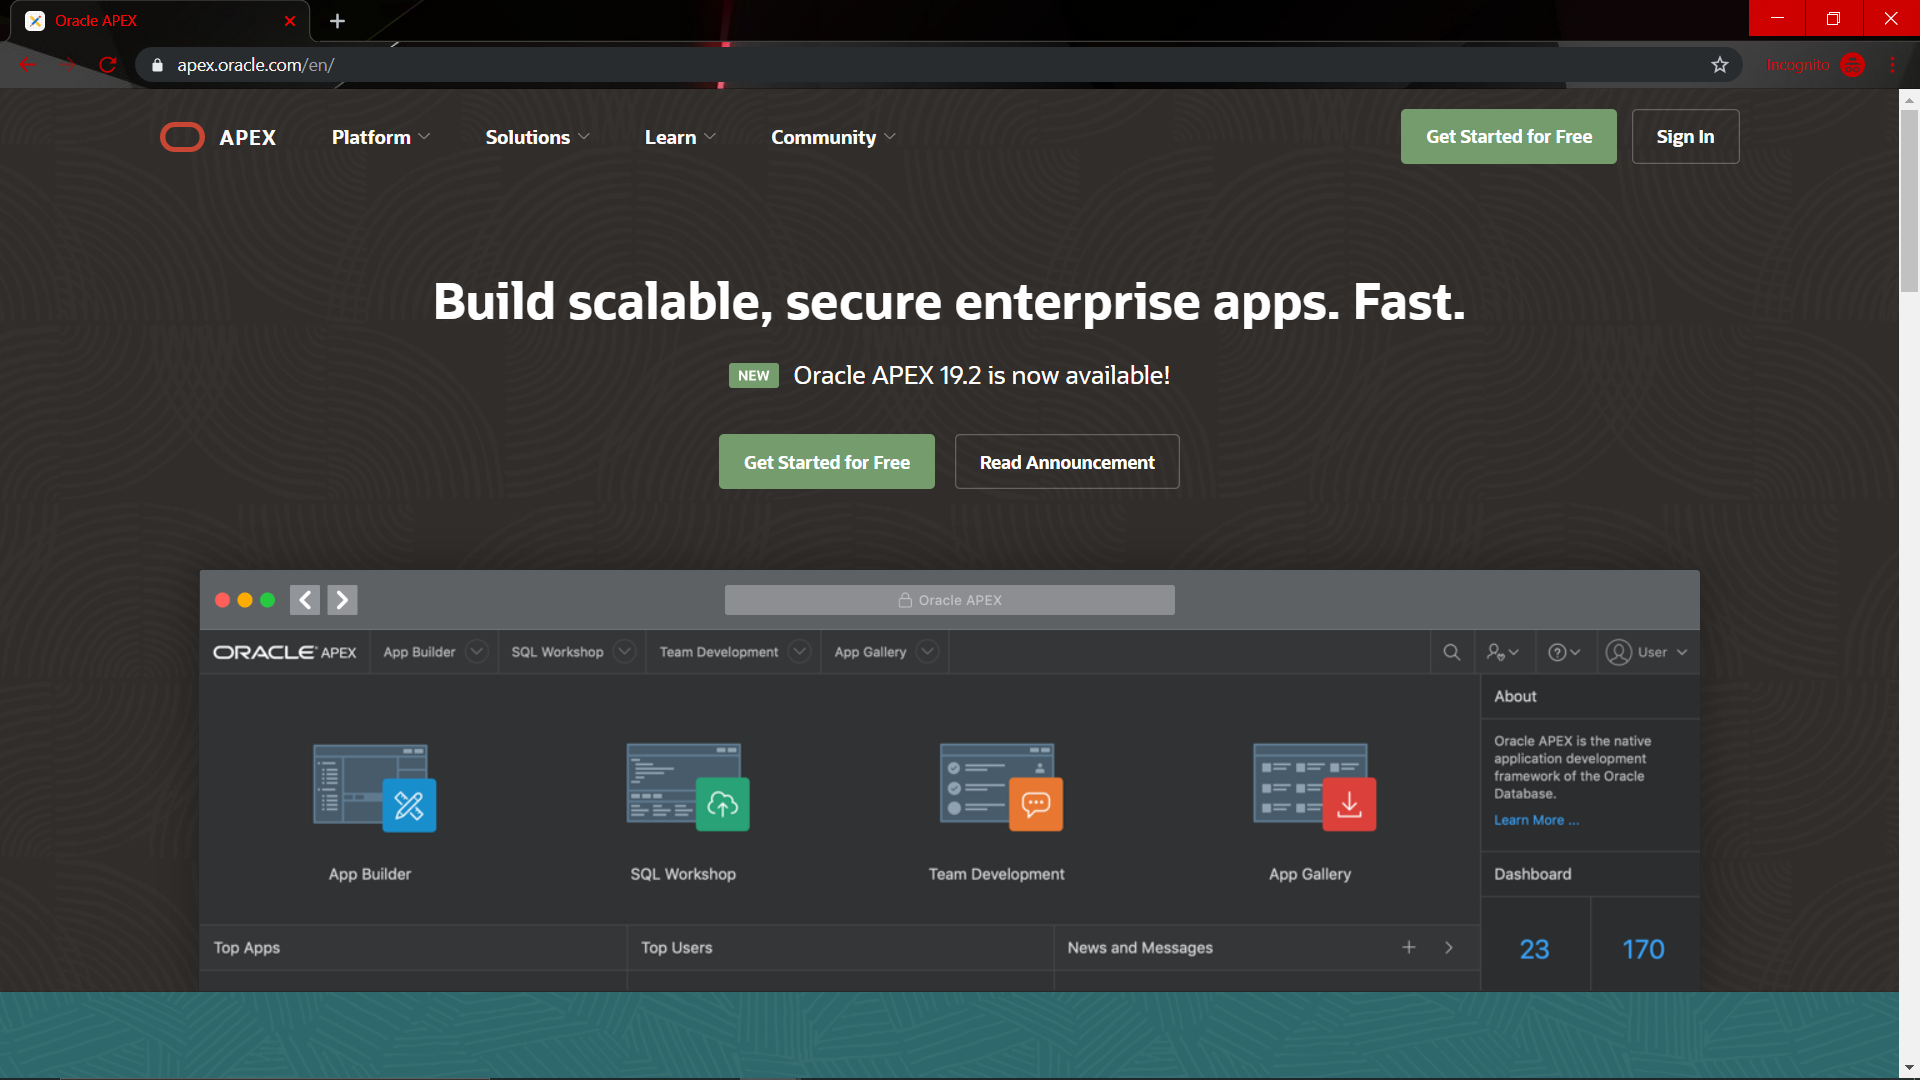
\includegraphics[scale=0.2]{Apex/0.png}
    \end{center}   
    \end{figure}
    
	\item Selanjutnya isi identificationnya, seperti gambar dibawah ini: 
	\begin{center}
    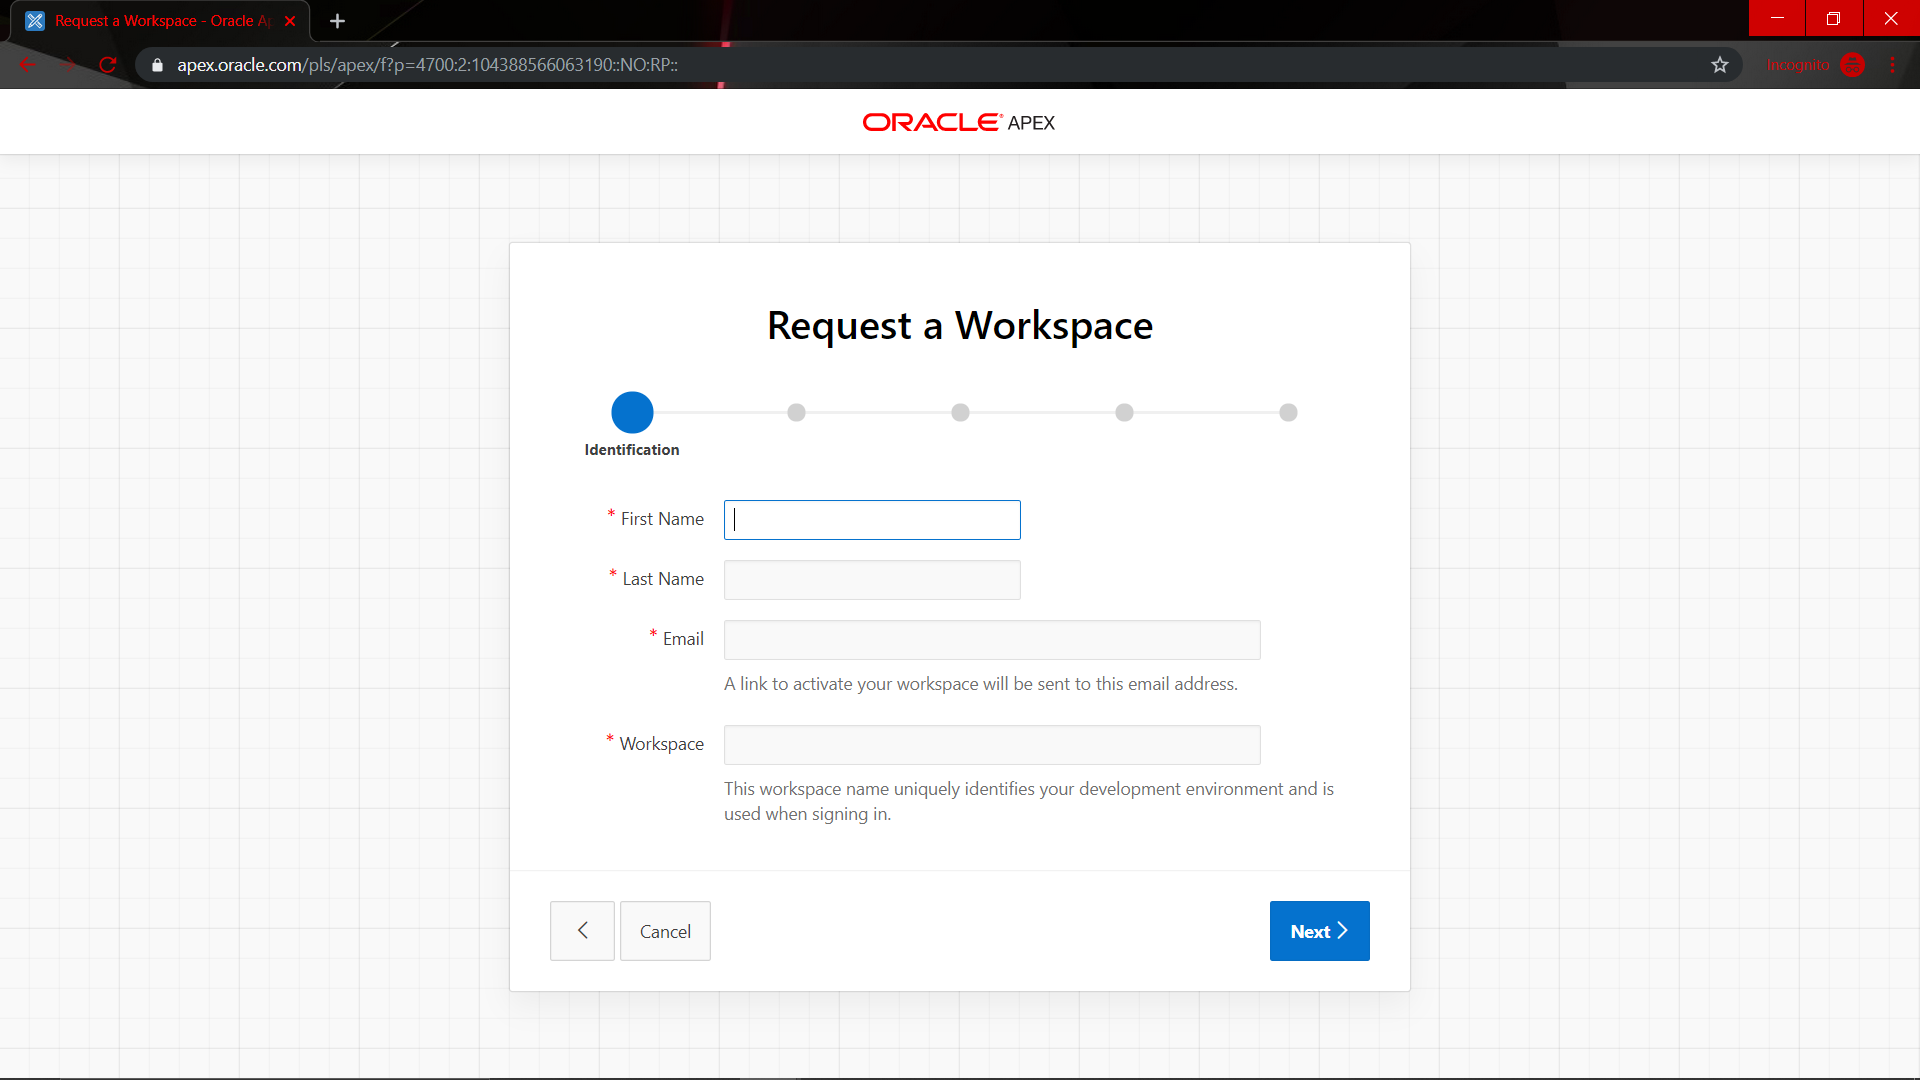
\includegraphics[scale=0.2]{Apex/1.png}
    \end{center}
    
	\item Setelah itu klik yes pada surveynya, dapat dilihat seperti dibawah ini:
	\begin{center}
    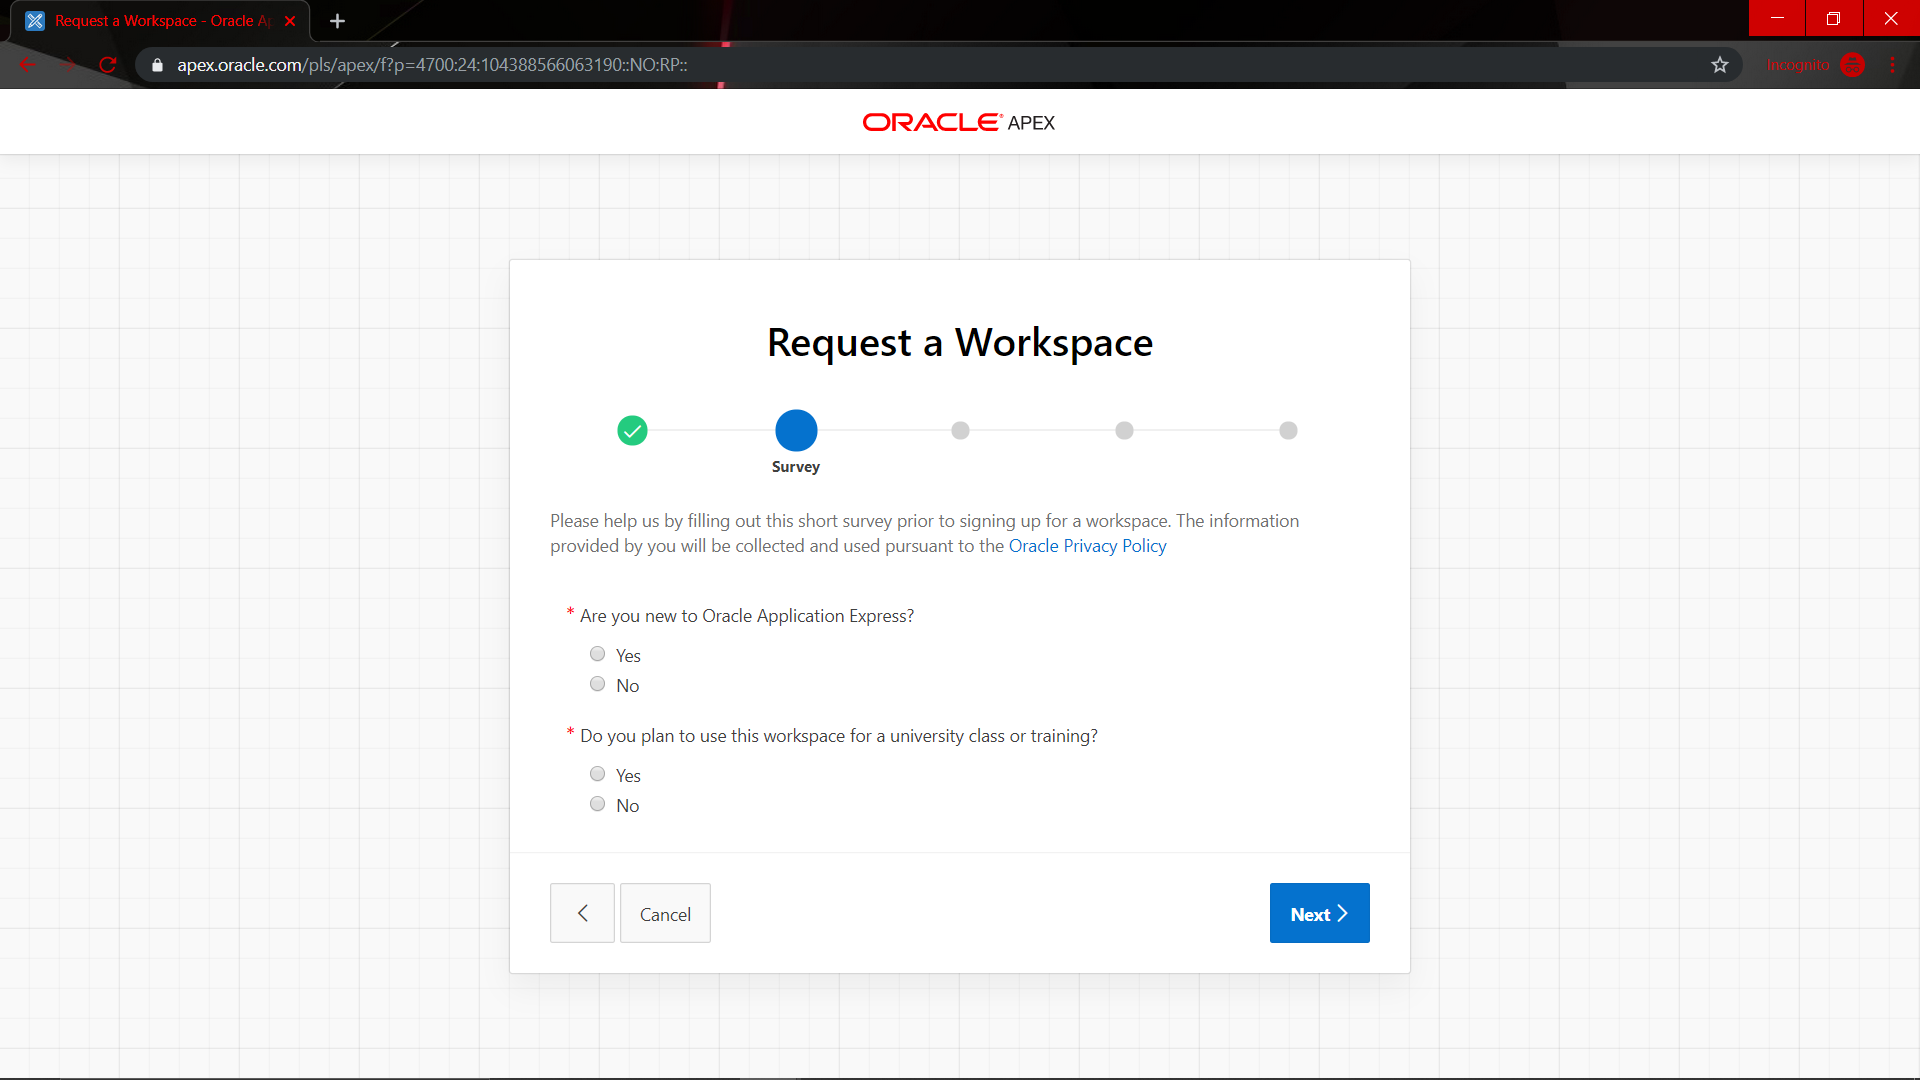
\includegraphics[scale=0.2]{Apex/2.png}
    \end{center}
	
	\item Lalu isi justificationnya 
	\begin{center}
    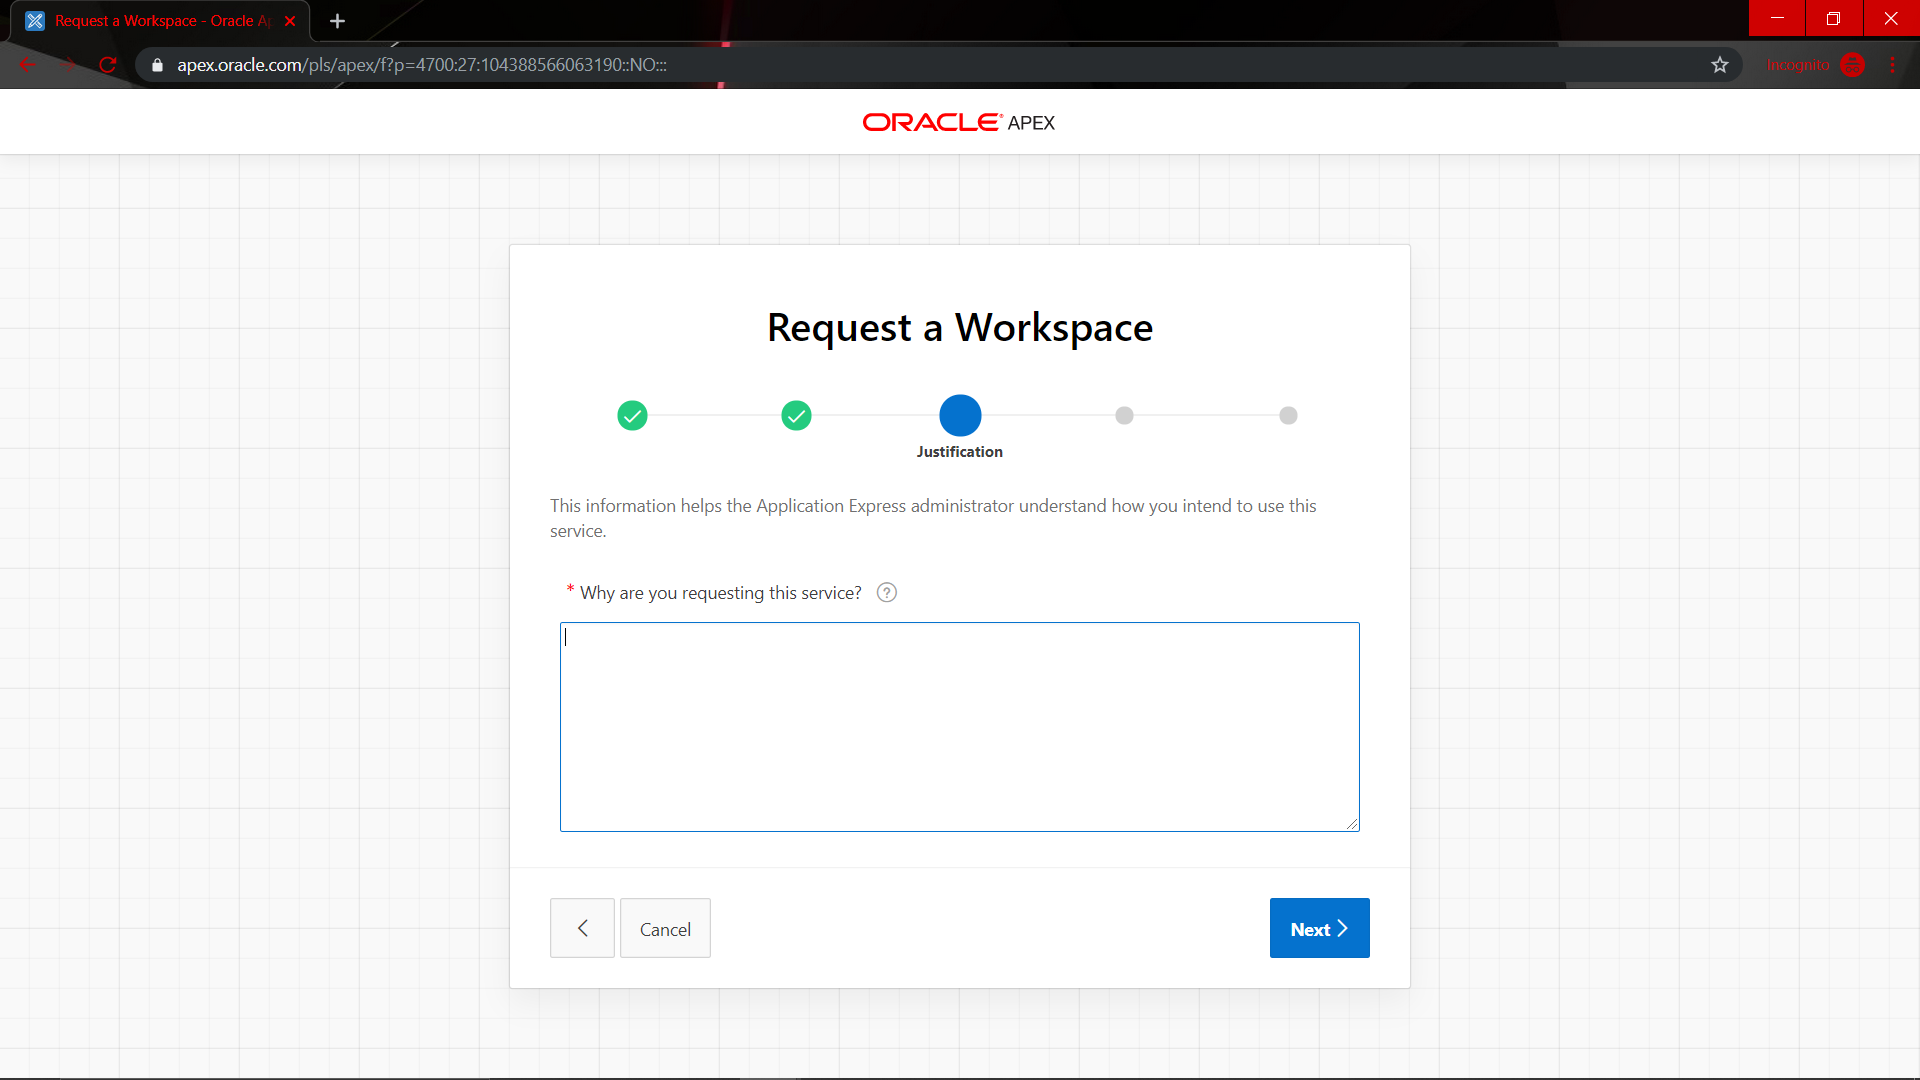
\includegraphics[scale=0.2]{Apex/3.png}
    \end{center}
    
	\item Kemudian centang I accept the terms pada agremeent
    \begin{center}
    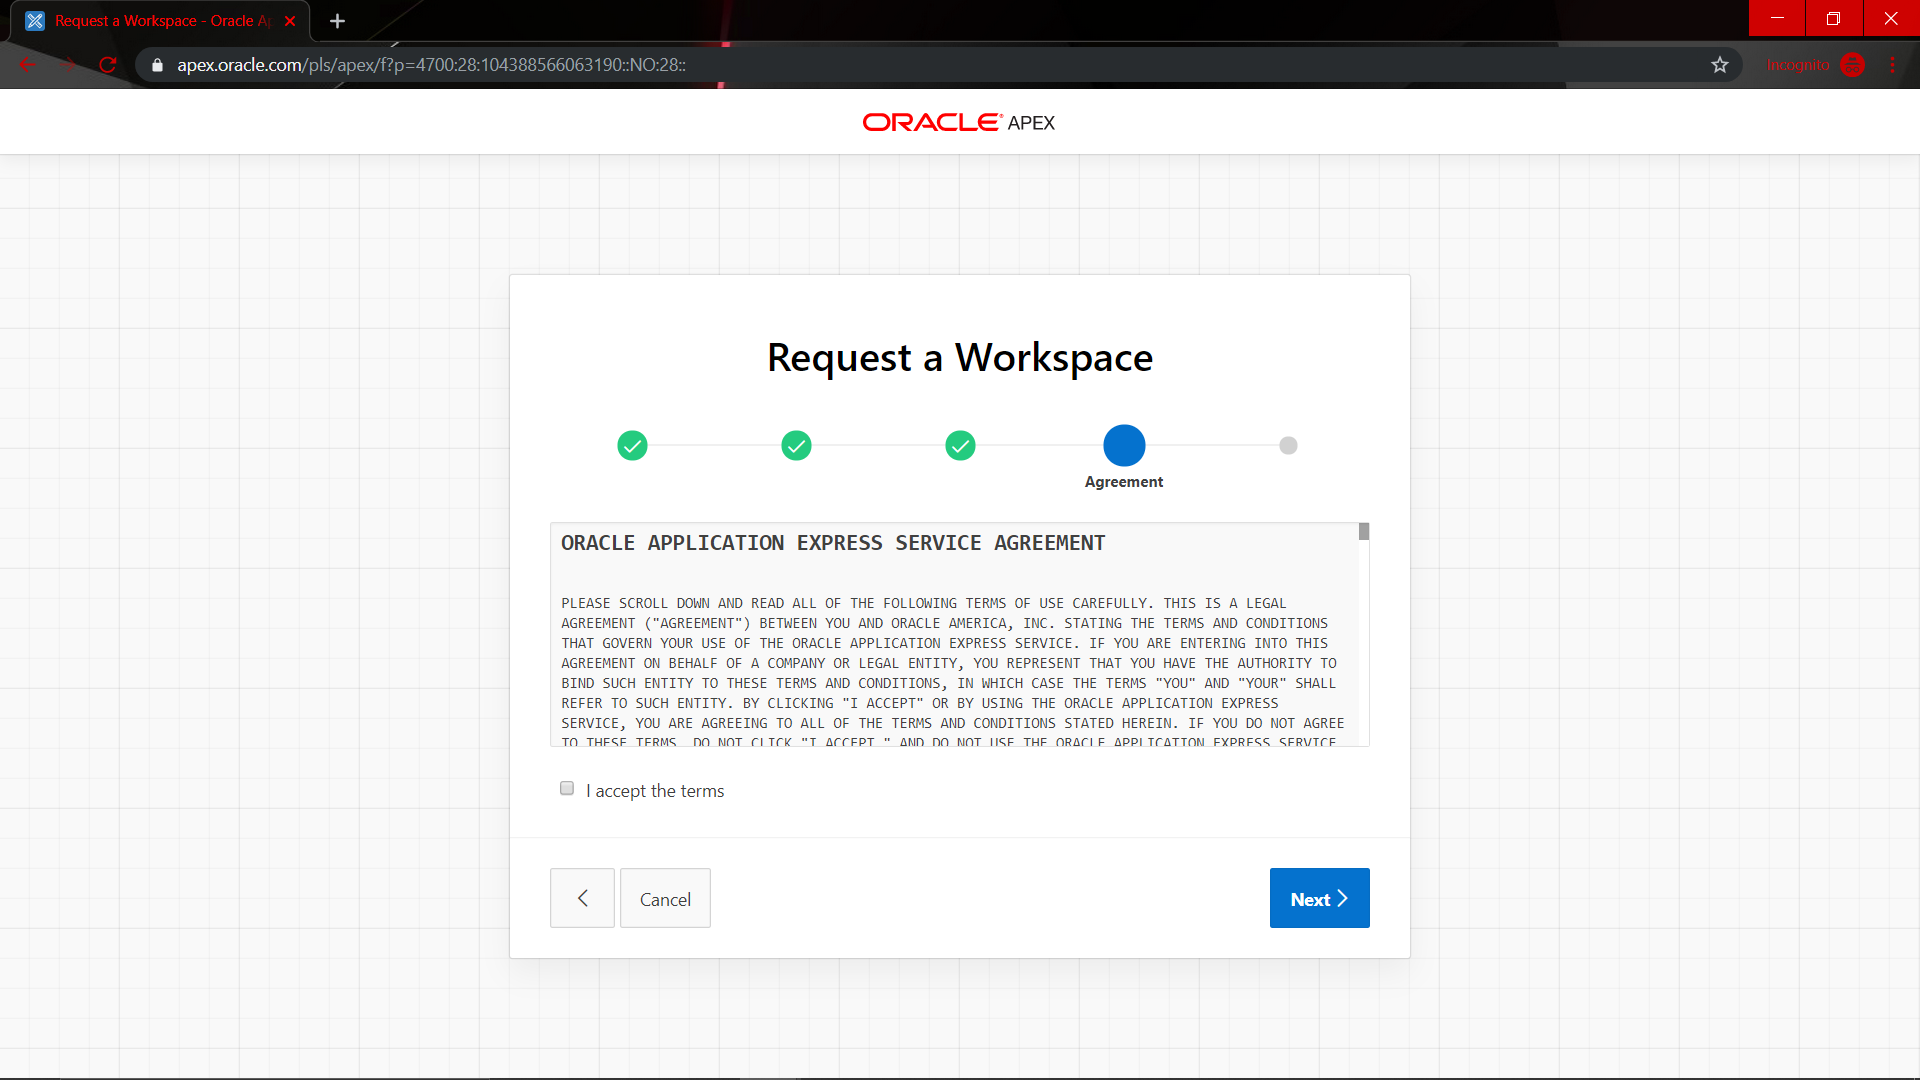
\includegraphics[scale=0.2]{Apex/4.png}
    \end{center}
	
	\item Setelah semuanya diisi, lalu pada bagian confirm klik submit request
	\begin{center}
    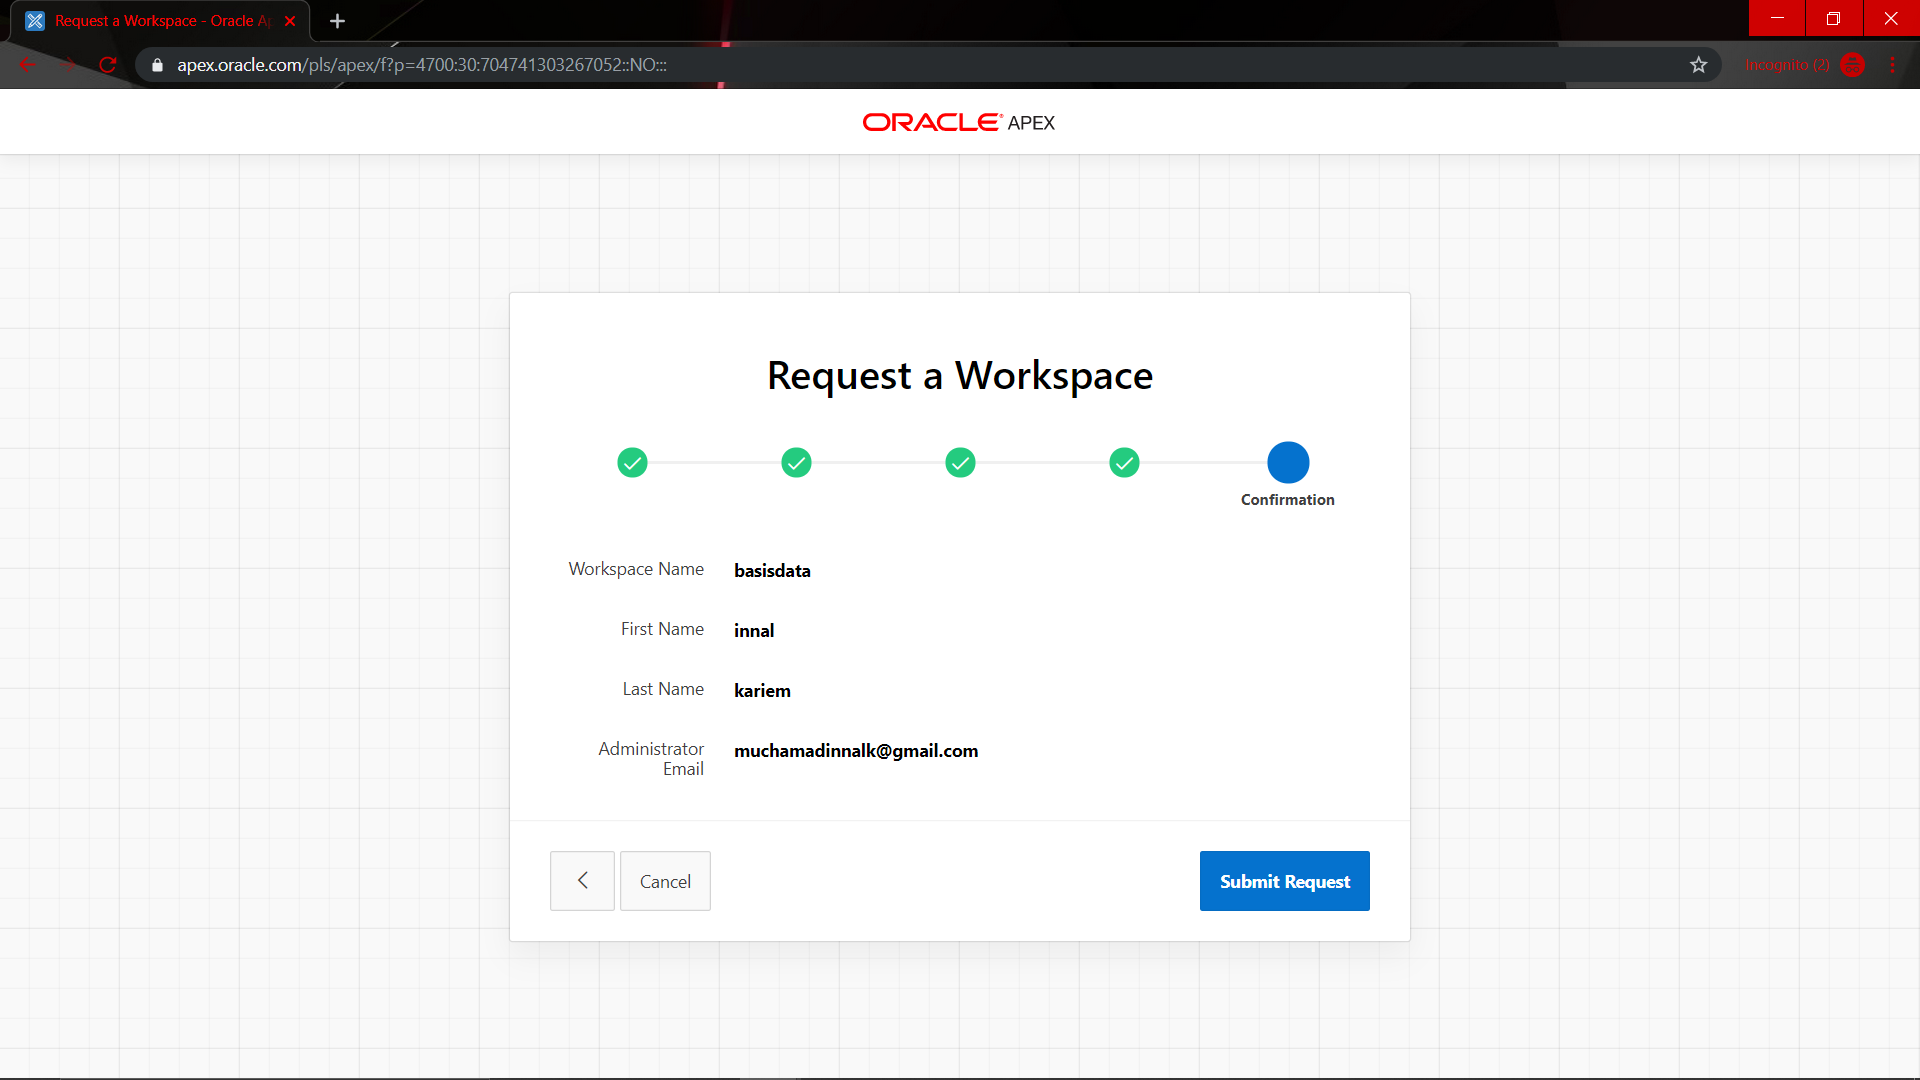
\includegraphics[scale=0.2]{Apex/5.png}
    \end{center}
	
	\item Selanjutnya buka email dan tunggu confirmasi diemail kita, lalu klik creat workspace 
	\begin{center}
    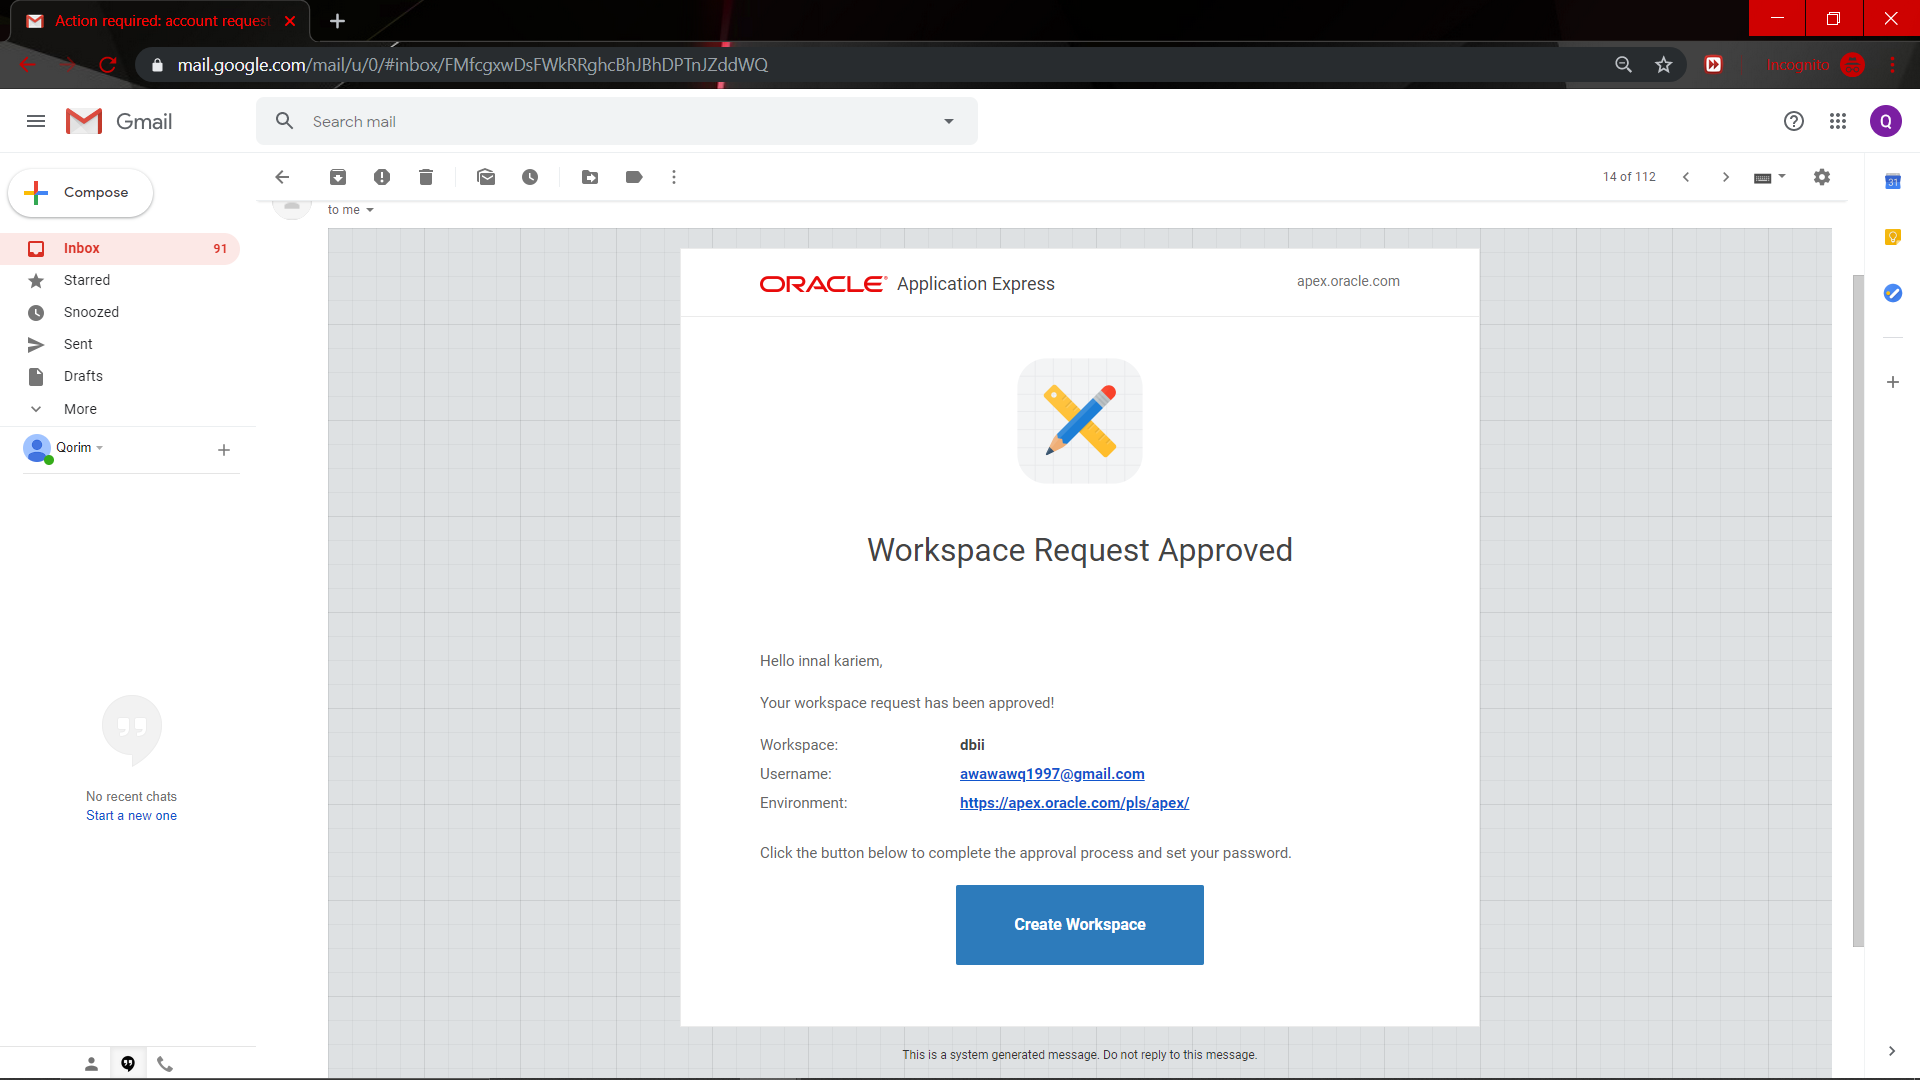
\includegraphics[scale=0.2]{Apex/6.png}
    \end{center}
	
	\item Lalu akan muncul Workspace Succesfully seperti gambar dibawah ini dan kllik continue to sign in screen
	\begin{center}
    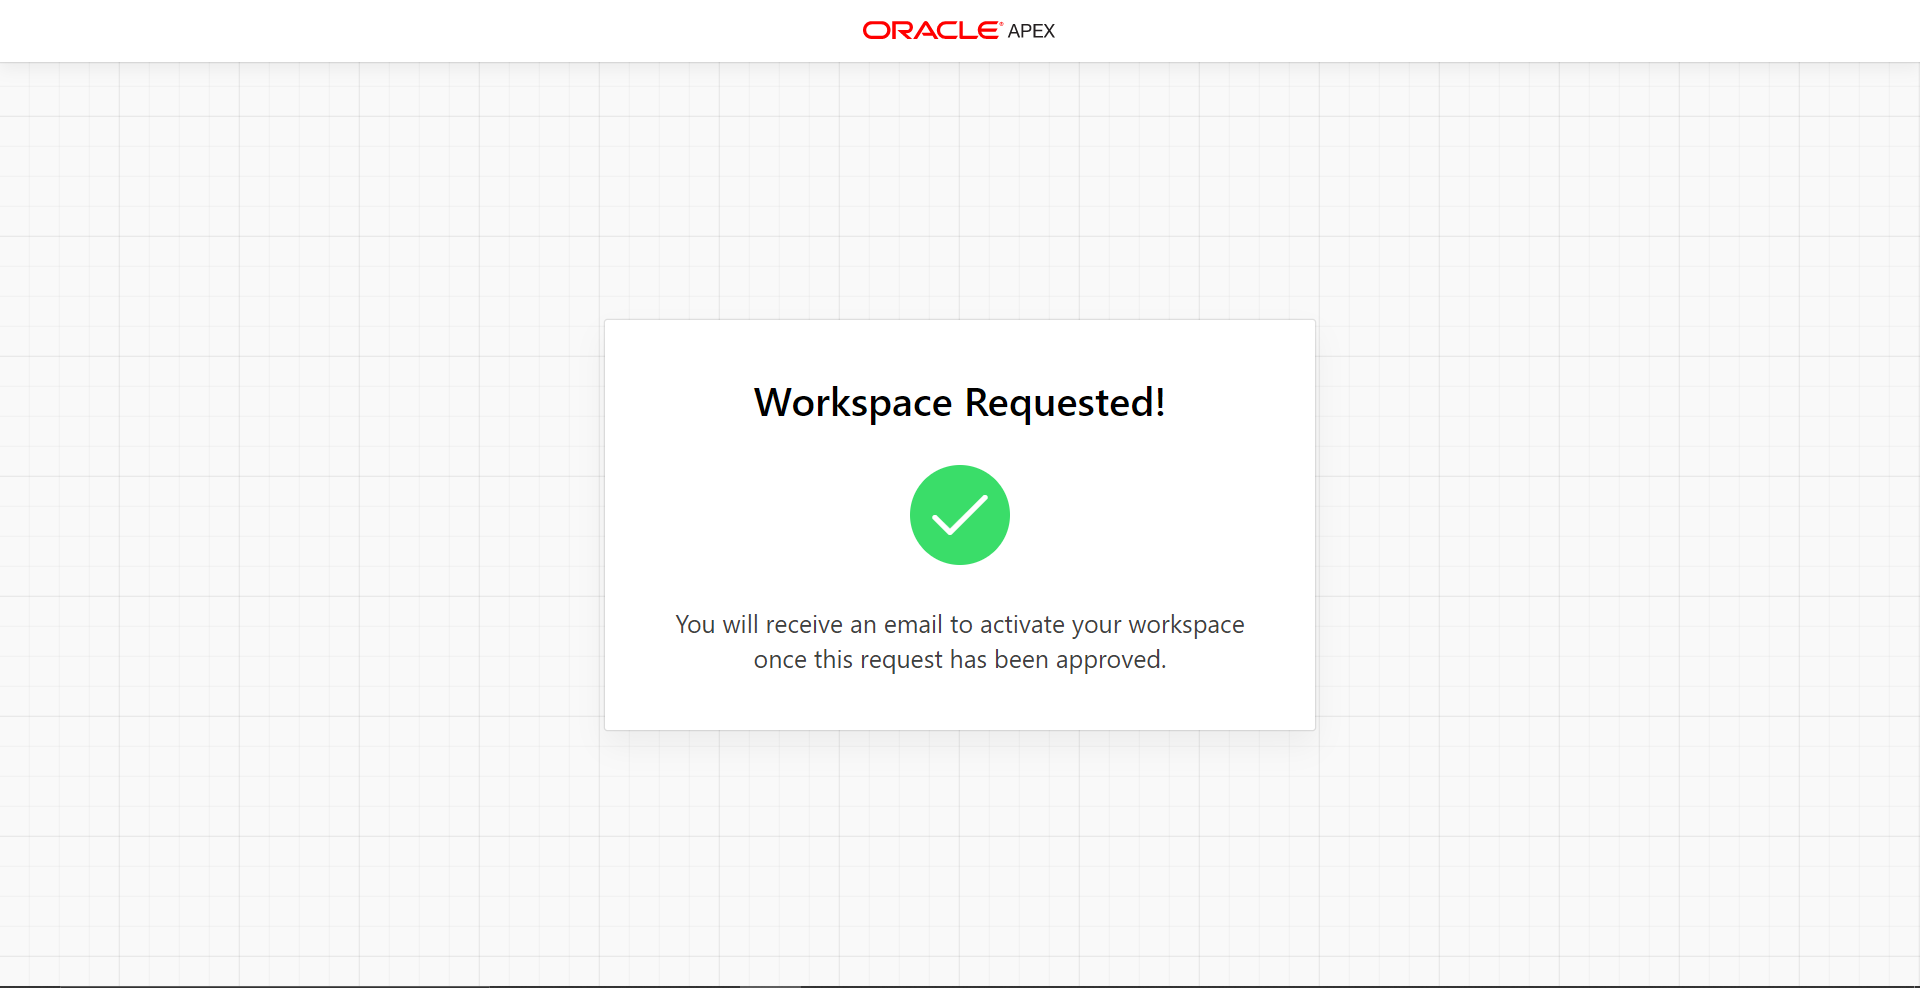
\includegraphics[scale=0.2]{Apex/7.png}
    \end{center}
	
	\item Setelah itu kita akan disuruh ganti password baru, seperti gambar dibawah ini
	\begin{center}
    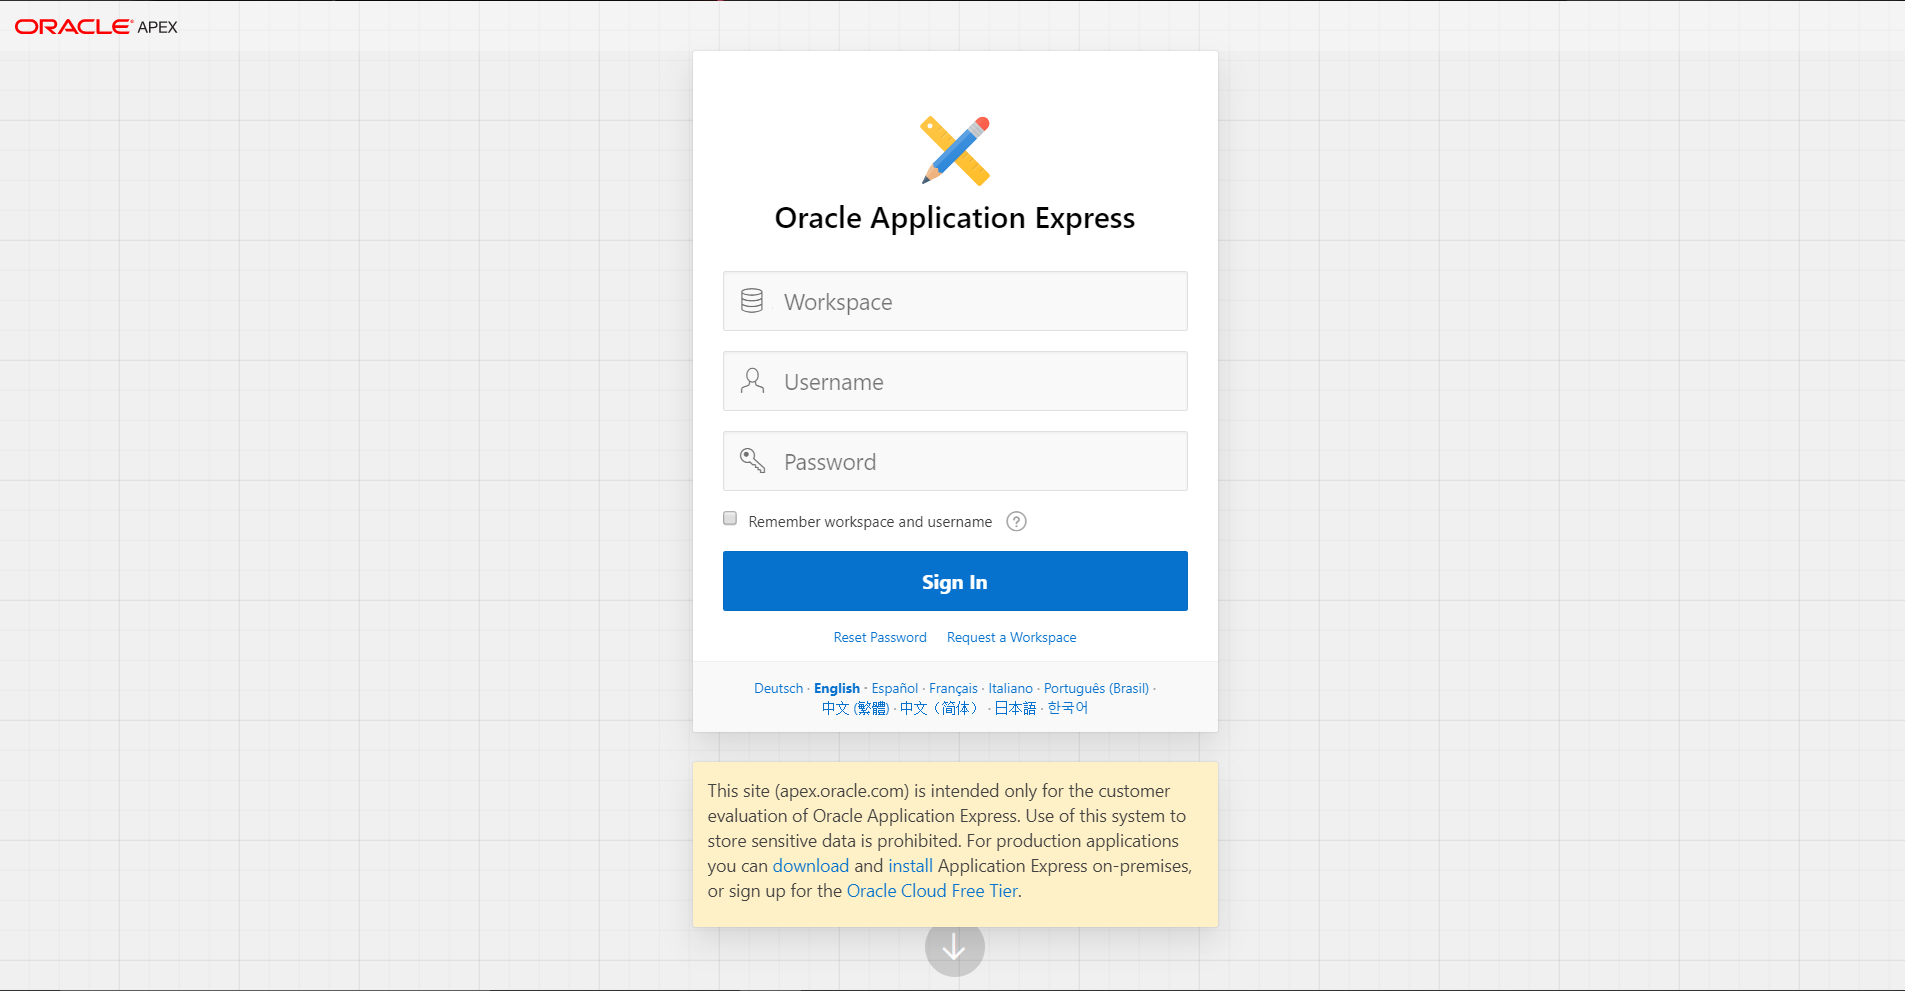
\includegraphics[scale=0.2]{Apex/8.png}
    \end{center}
	
	\item Kemudian setelah ganti password kita akan mucul ke halaman utama, Lalu klik SQL Workshop, kemudian pilih Utilities dan klik Data workhop, dapat dilihat seperti gambar dibawah ini :
	\begin{center}
    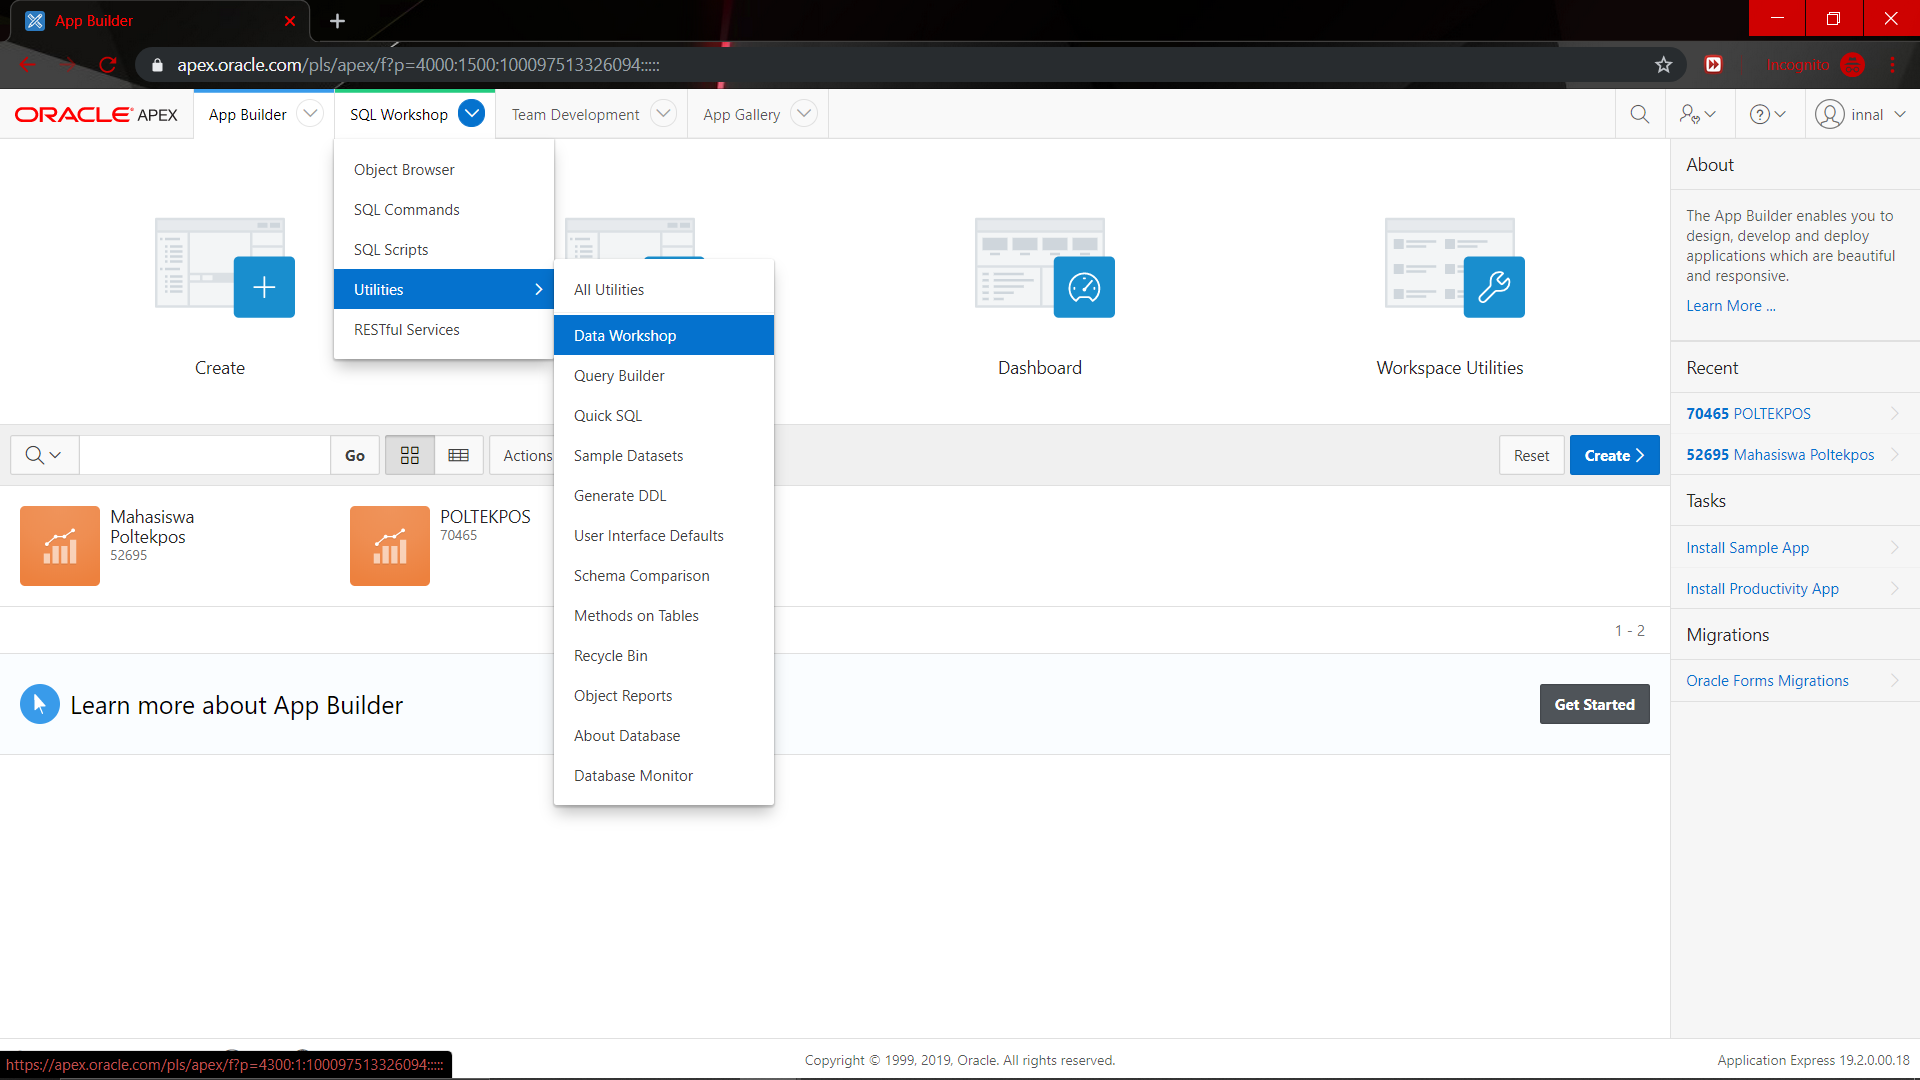
\includegraphics[scale=0.2]{Apex/48.png}
    \end{center}
	
	\item Selanjutnya klik load data, lalu pilih file excel yang akan diimport, kemudian open, seperti dibawah ini
	\begin{center}
    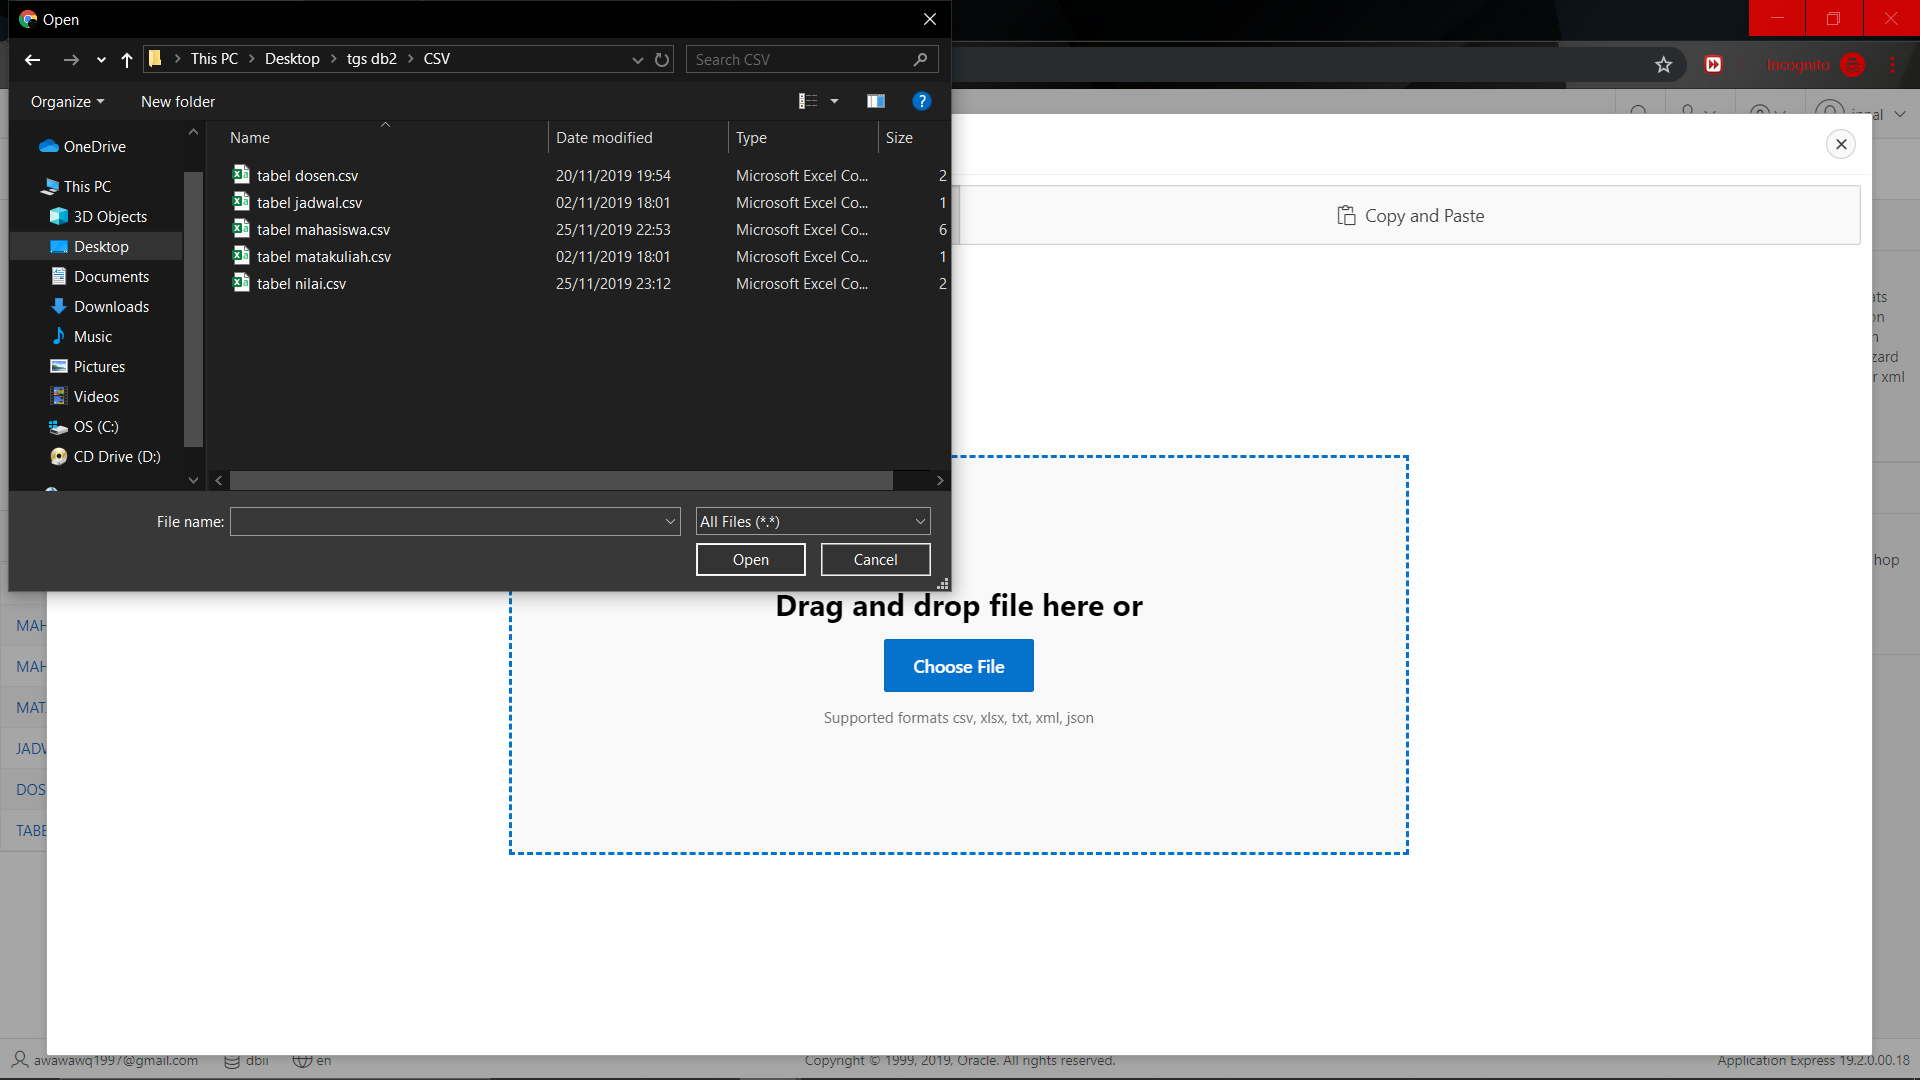
\includegraphics[scale=0.2]{Apex/49.png}
    \end{center}
    
	\item jika sudah masuk ke filenya, maka akan mucul seperti gambar dibawah ini, lalu isikan tabel name dan enter kemudian klik configure dan save change
	\begin{center}
    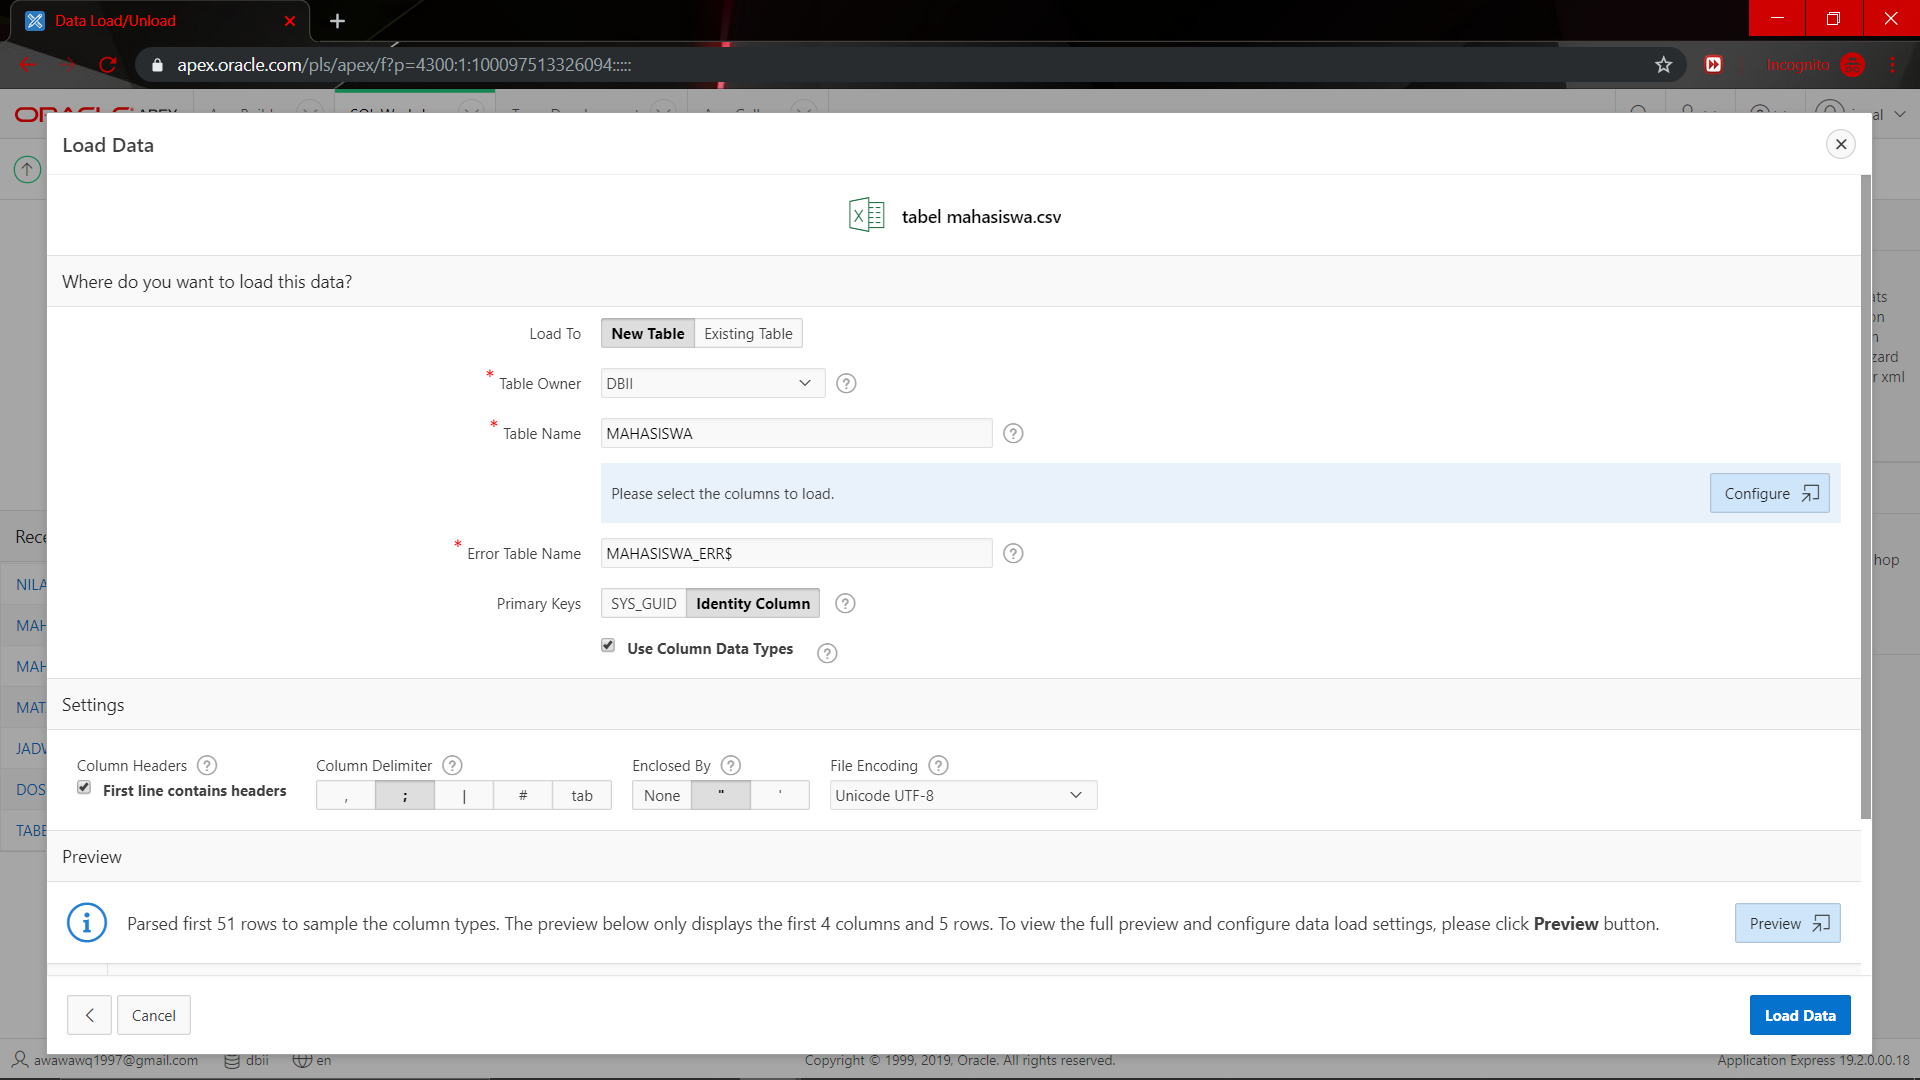
\includegraphics[scale=0.2]{Apex/50.png}
    \end{center}
    
    \item kemudian klik load data dan setelah itu close, maka akan muncul seperti gambar dibawah ini. Importkan semua file excel yang sudah disiapkan seperti cara tadi.
	\begin{center}
    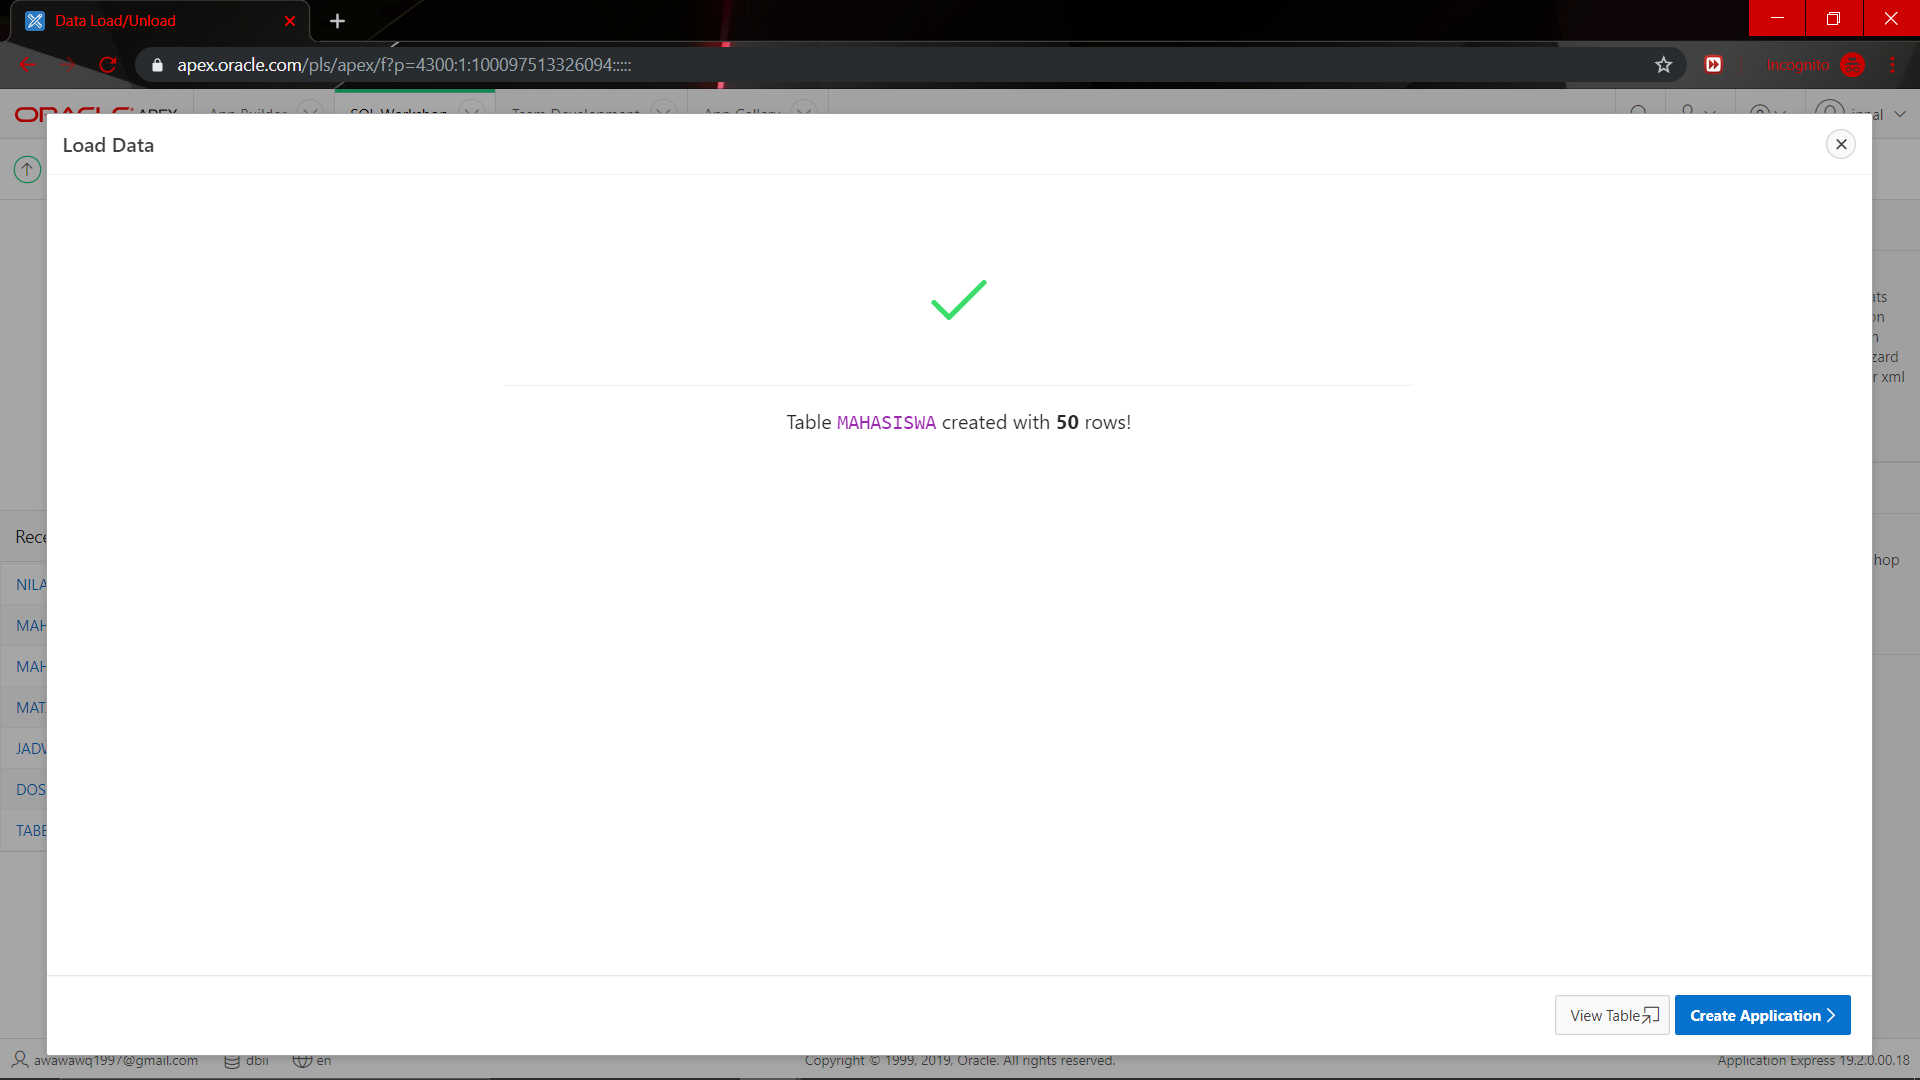
\includegraphics[scale=0.2]{Apex/58.png}
    \end{center}
    
    \item Selanjutnya relasikan antar tabel, yaitu dengan cara klik SQL workshop lalu pilih SQL command
	\begin{center}
    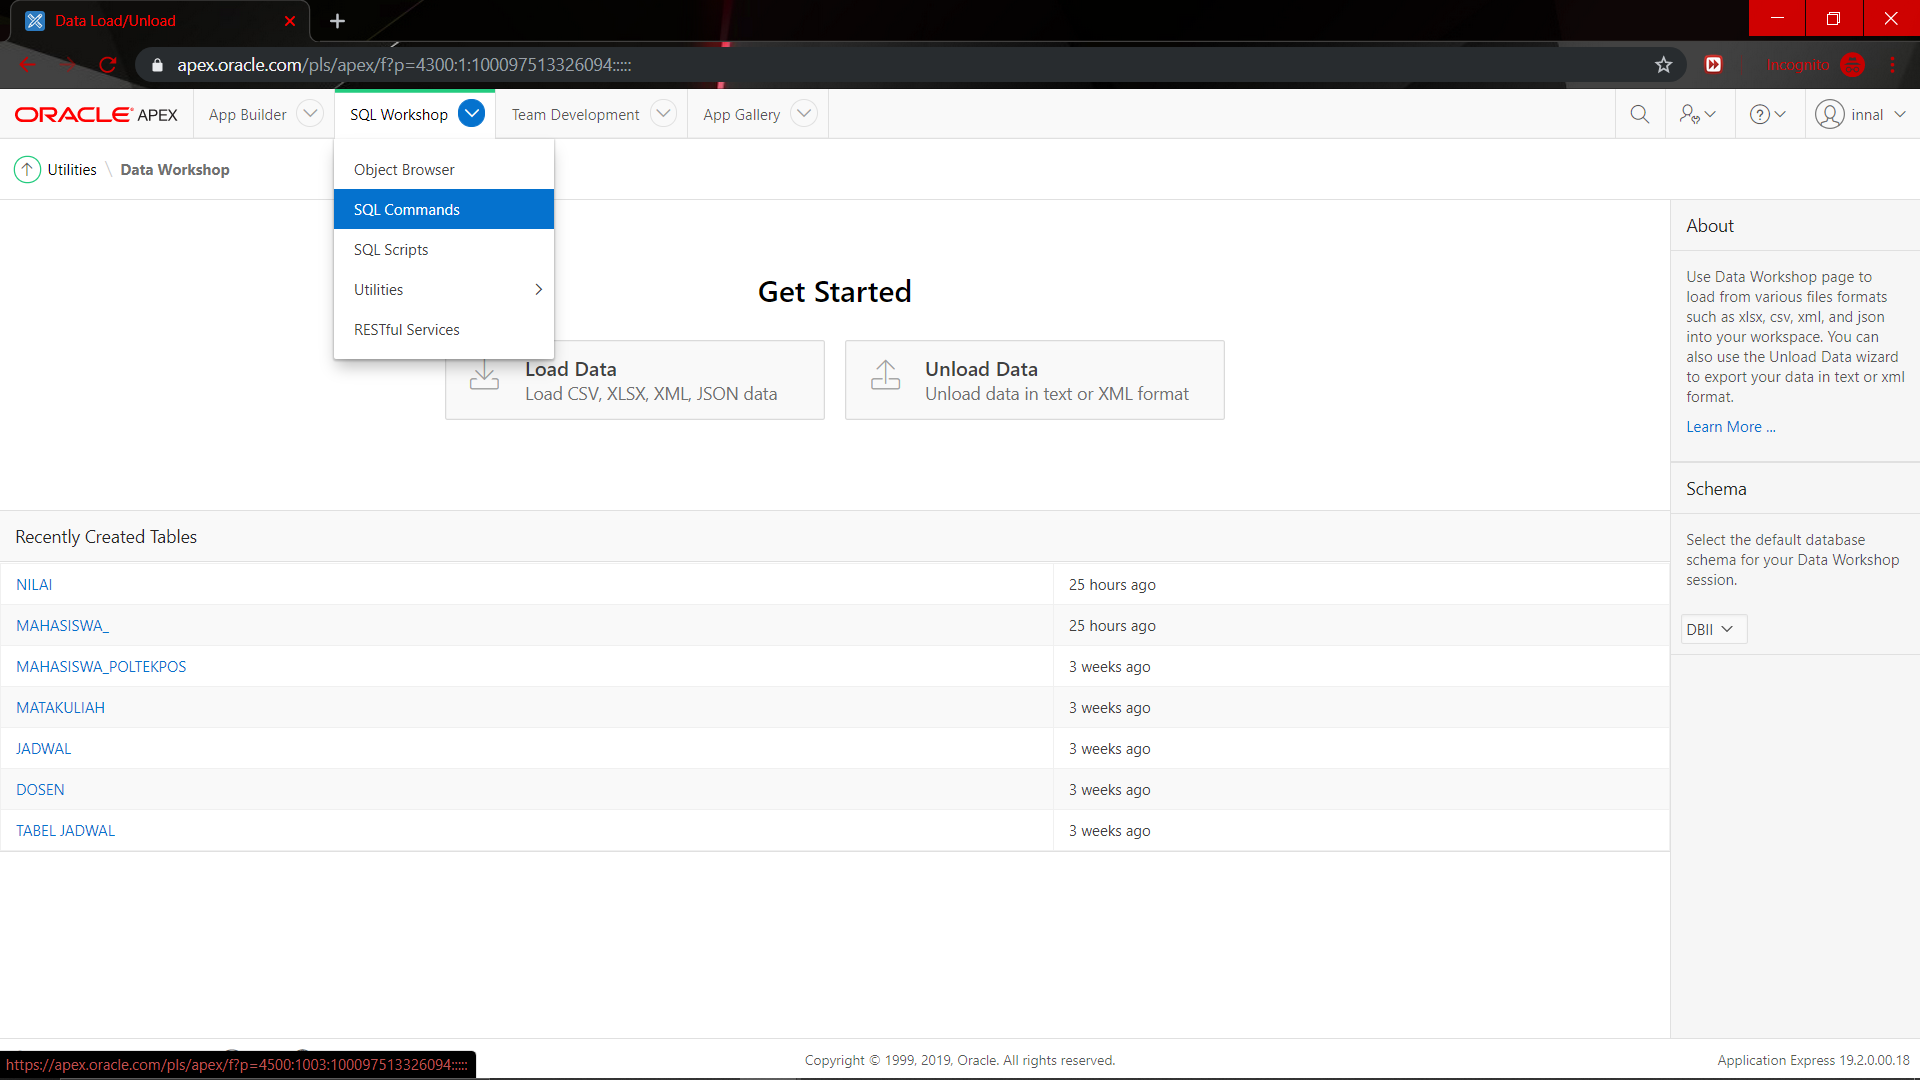
\includegraphics[scale=0.2]{Apex/59.png}
    \end{center}
    
    \item kemudian ketik seperti dibawah ini untuk menghapus kolom ID setiap tabel.
	\begin{center}
    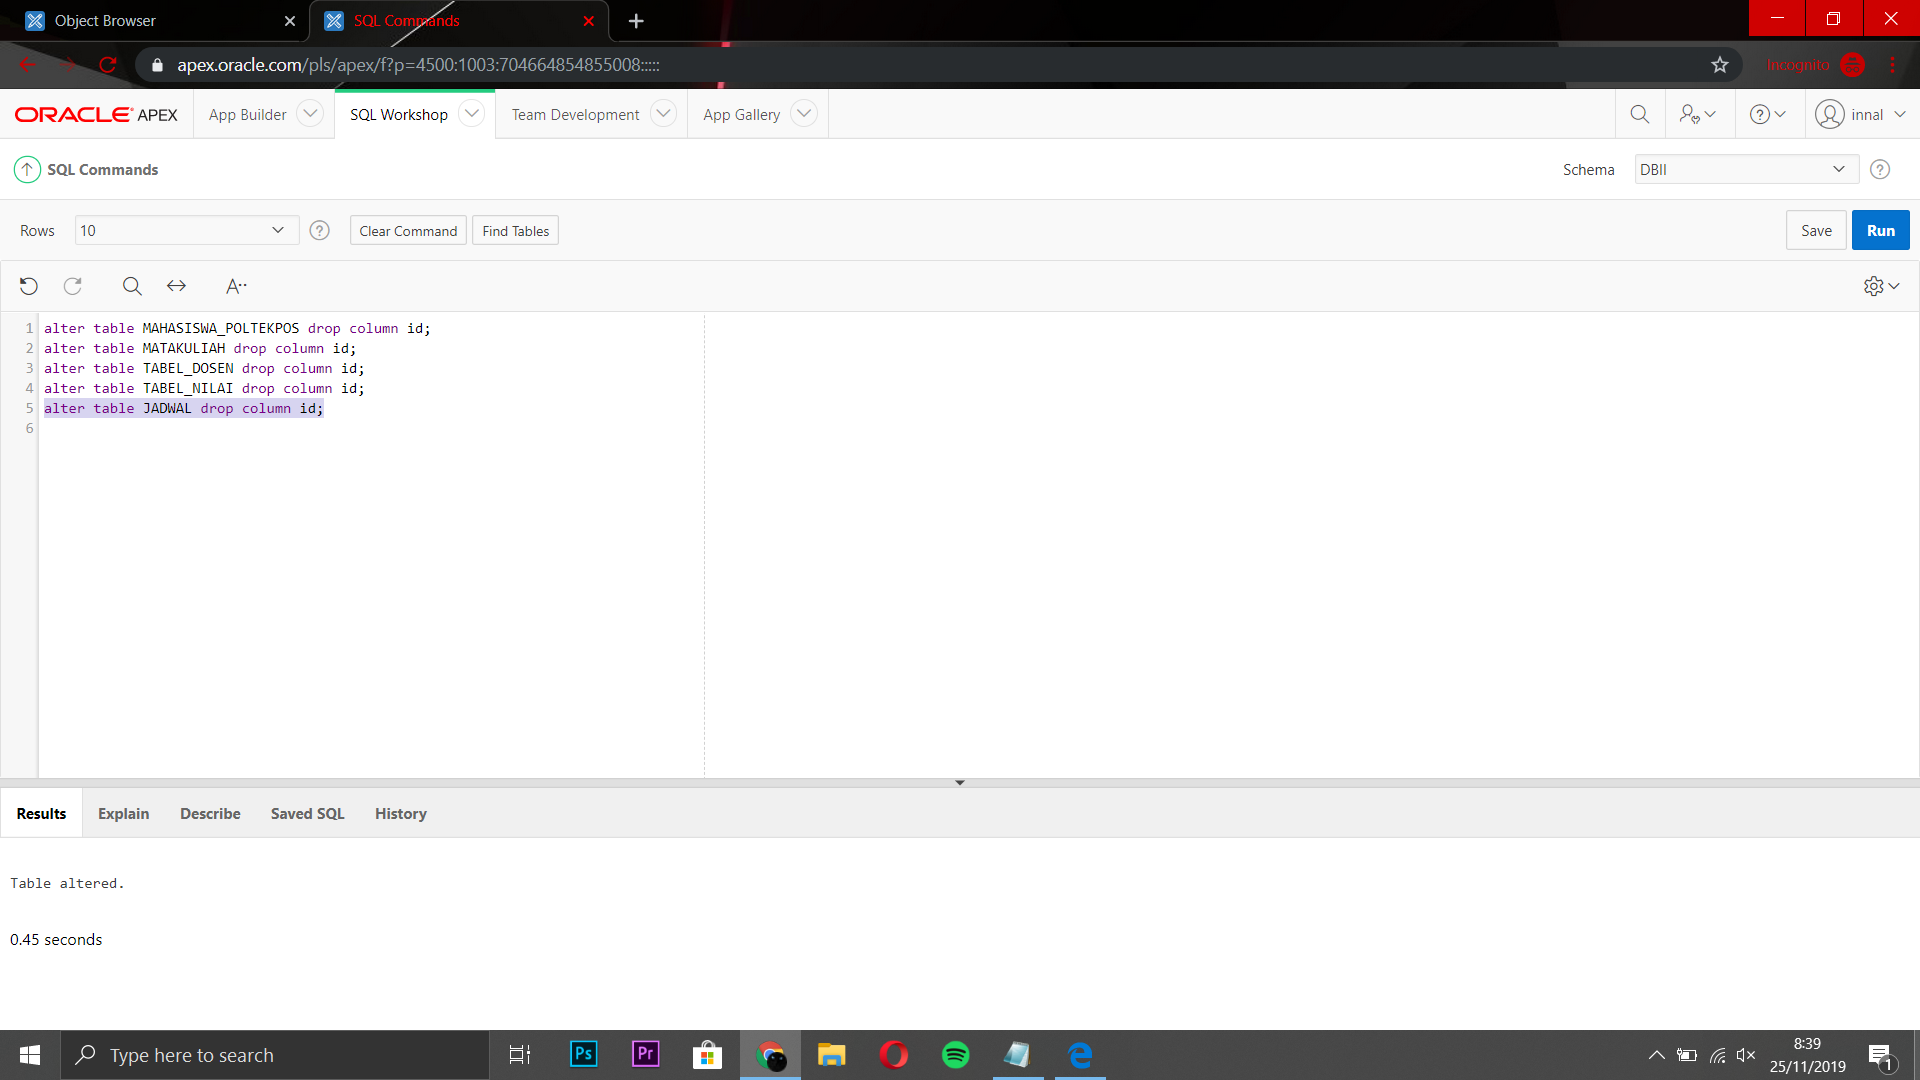
\includegraphics[scale=0.2]{Apex/61.png}
    \end{center}

    \item Setelah itu buat primary key pada tabel mahasiswa,dosen dan mata kuliah.Primary keynya harus bersifat unique, kemudian ketik seperti gambar dibawah ini pada SQL command
	\begin{center}
    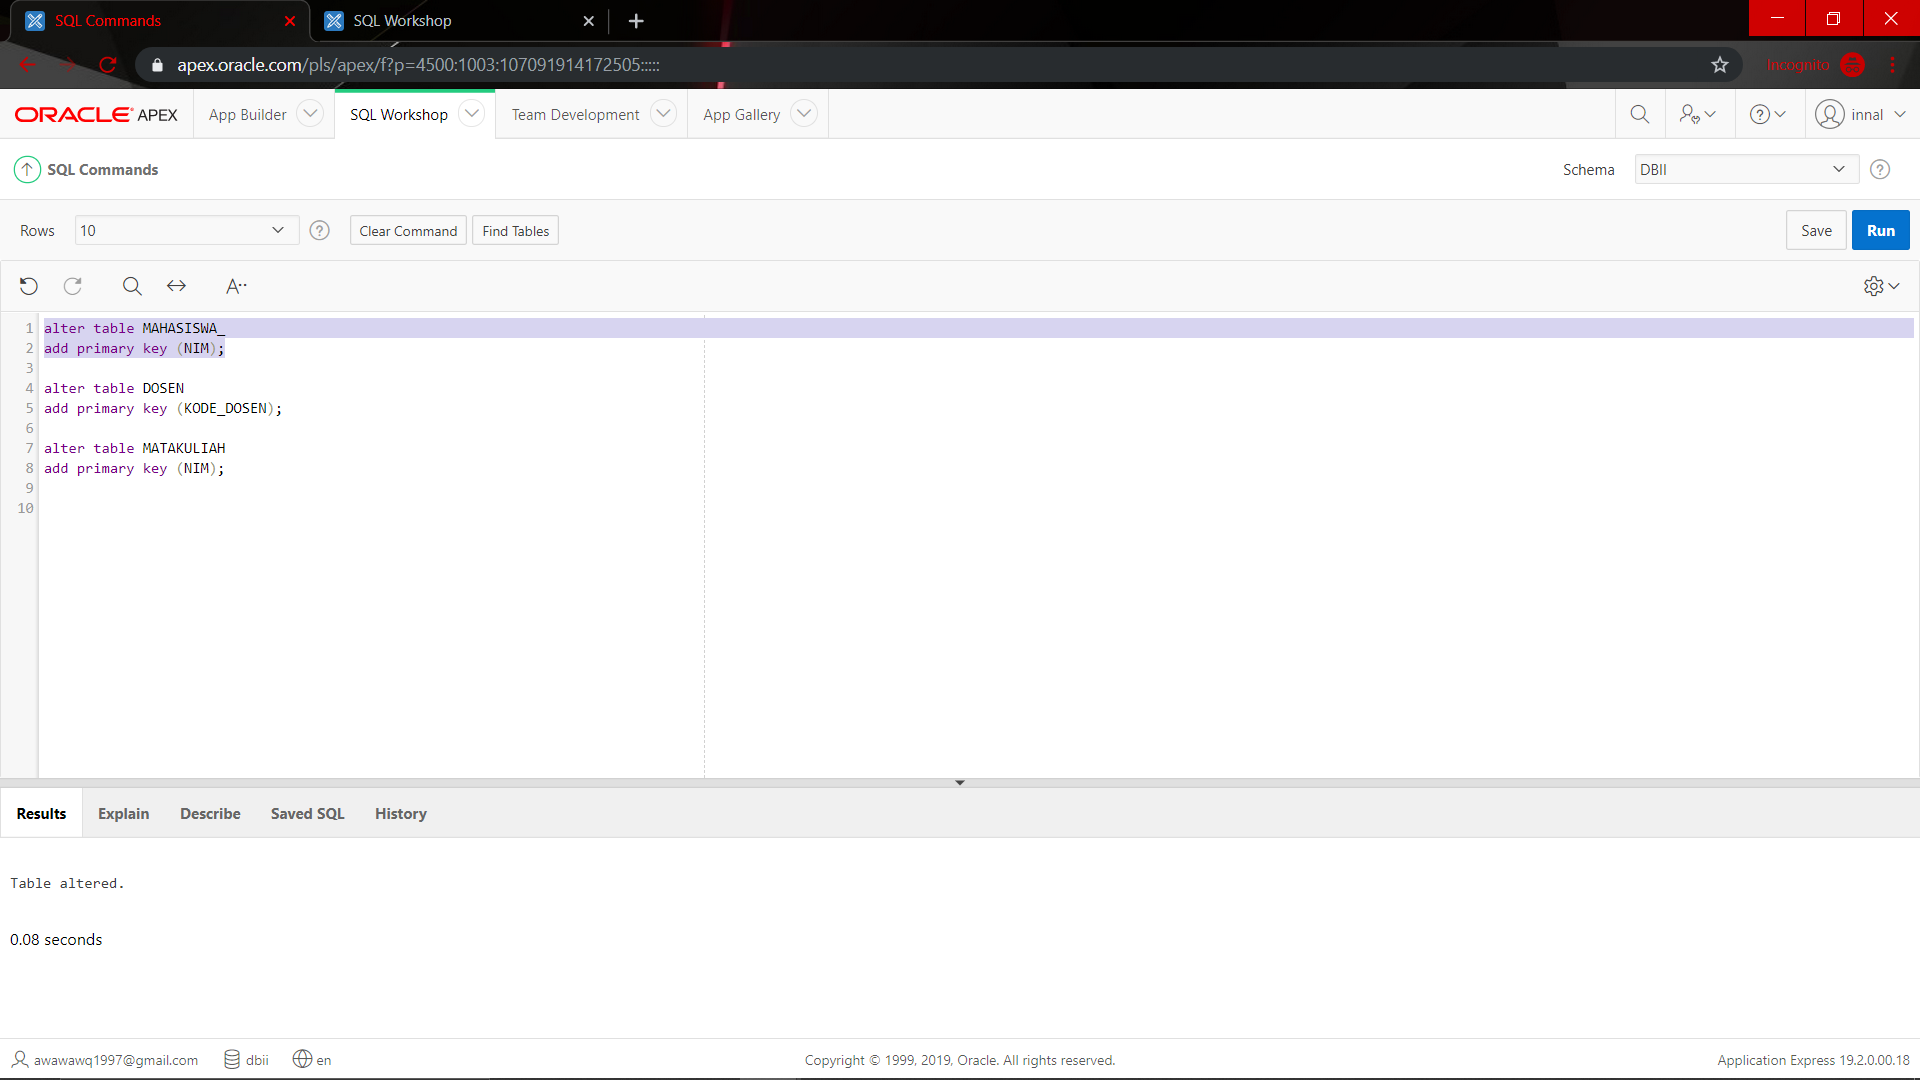
\includegraphics[scale=0.2]{Apex/62.png}
    \end{center}
    
    \item Setelah itu ketik lagi pada SQL Command seperti gambar dibawah ini, Lalu RUN
	\begin{center}
    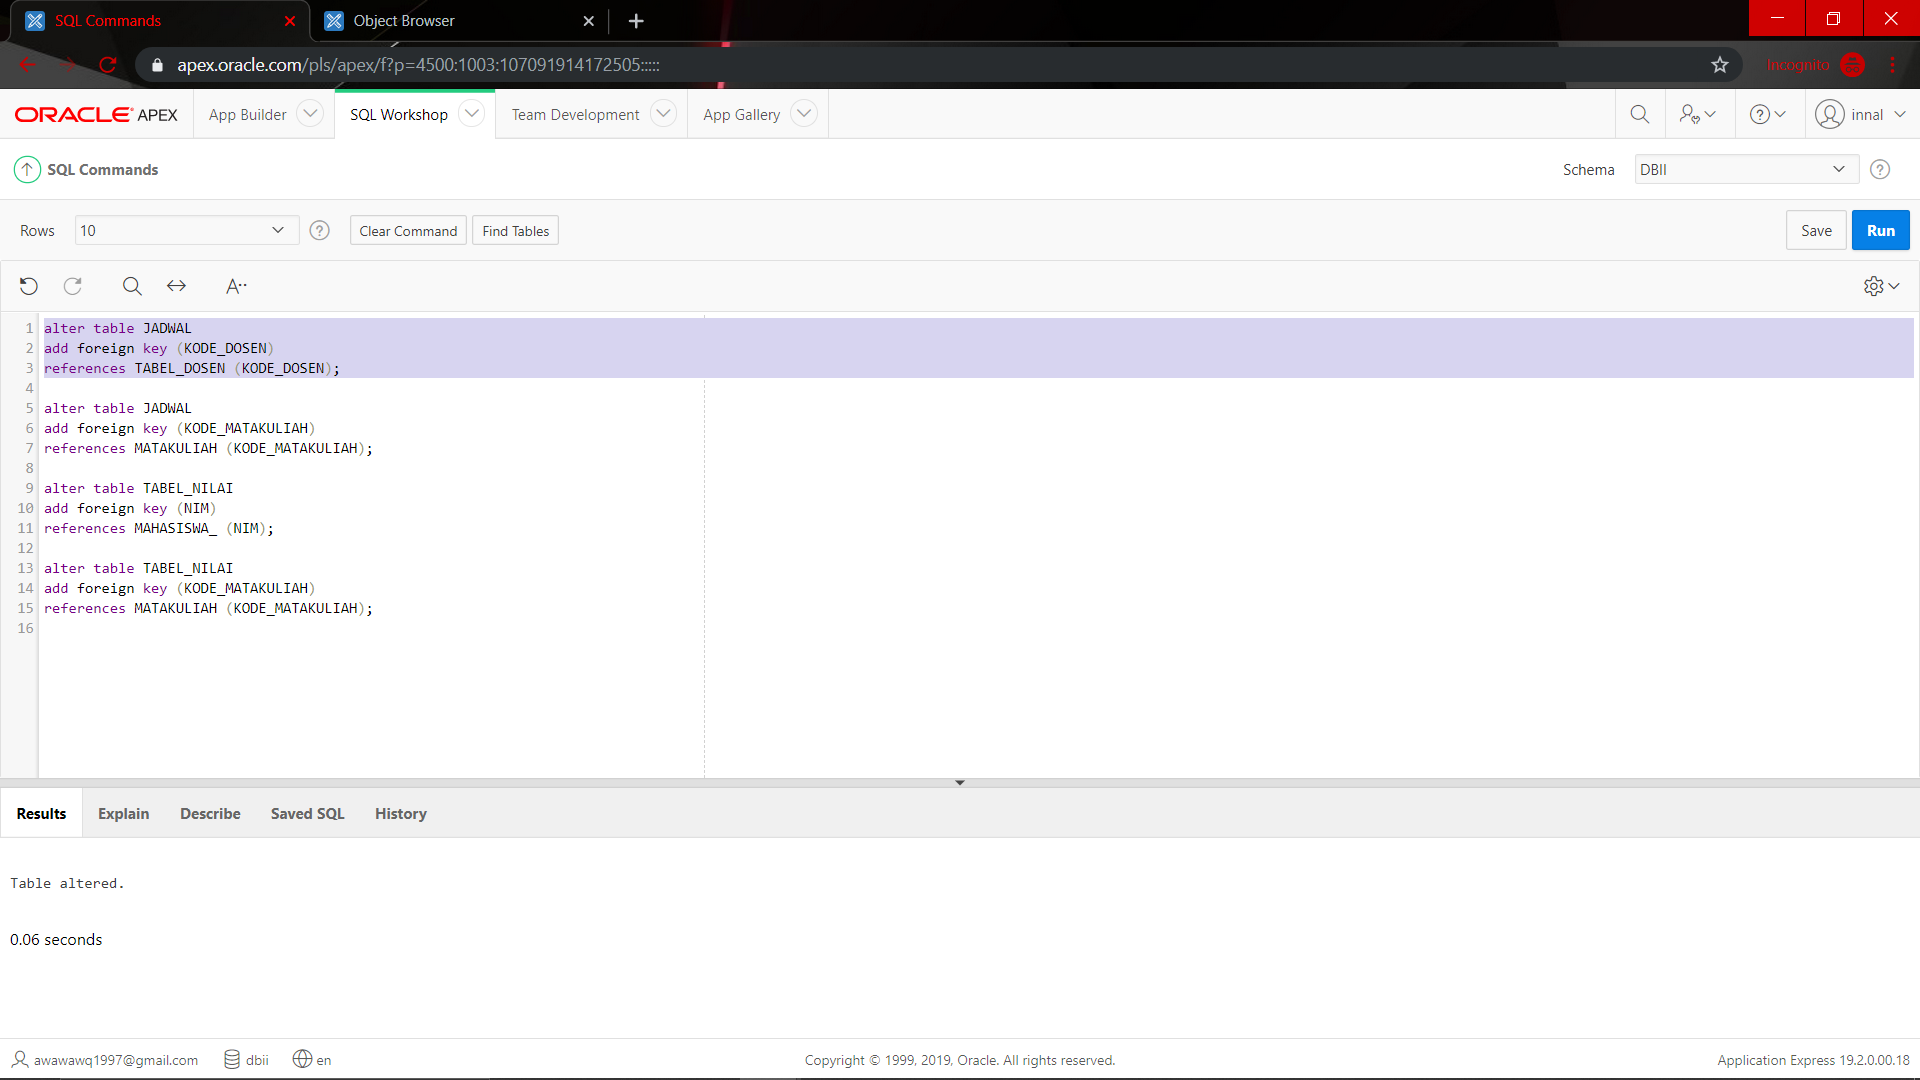
\includegraphics[scale=0.2]{Apex/63.png}
    \end{center}

    \item Kemudian klik app Builder dan klik create, Lalu klik new Application, seperti gambar dibawah ini
	\begin{center}
    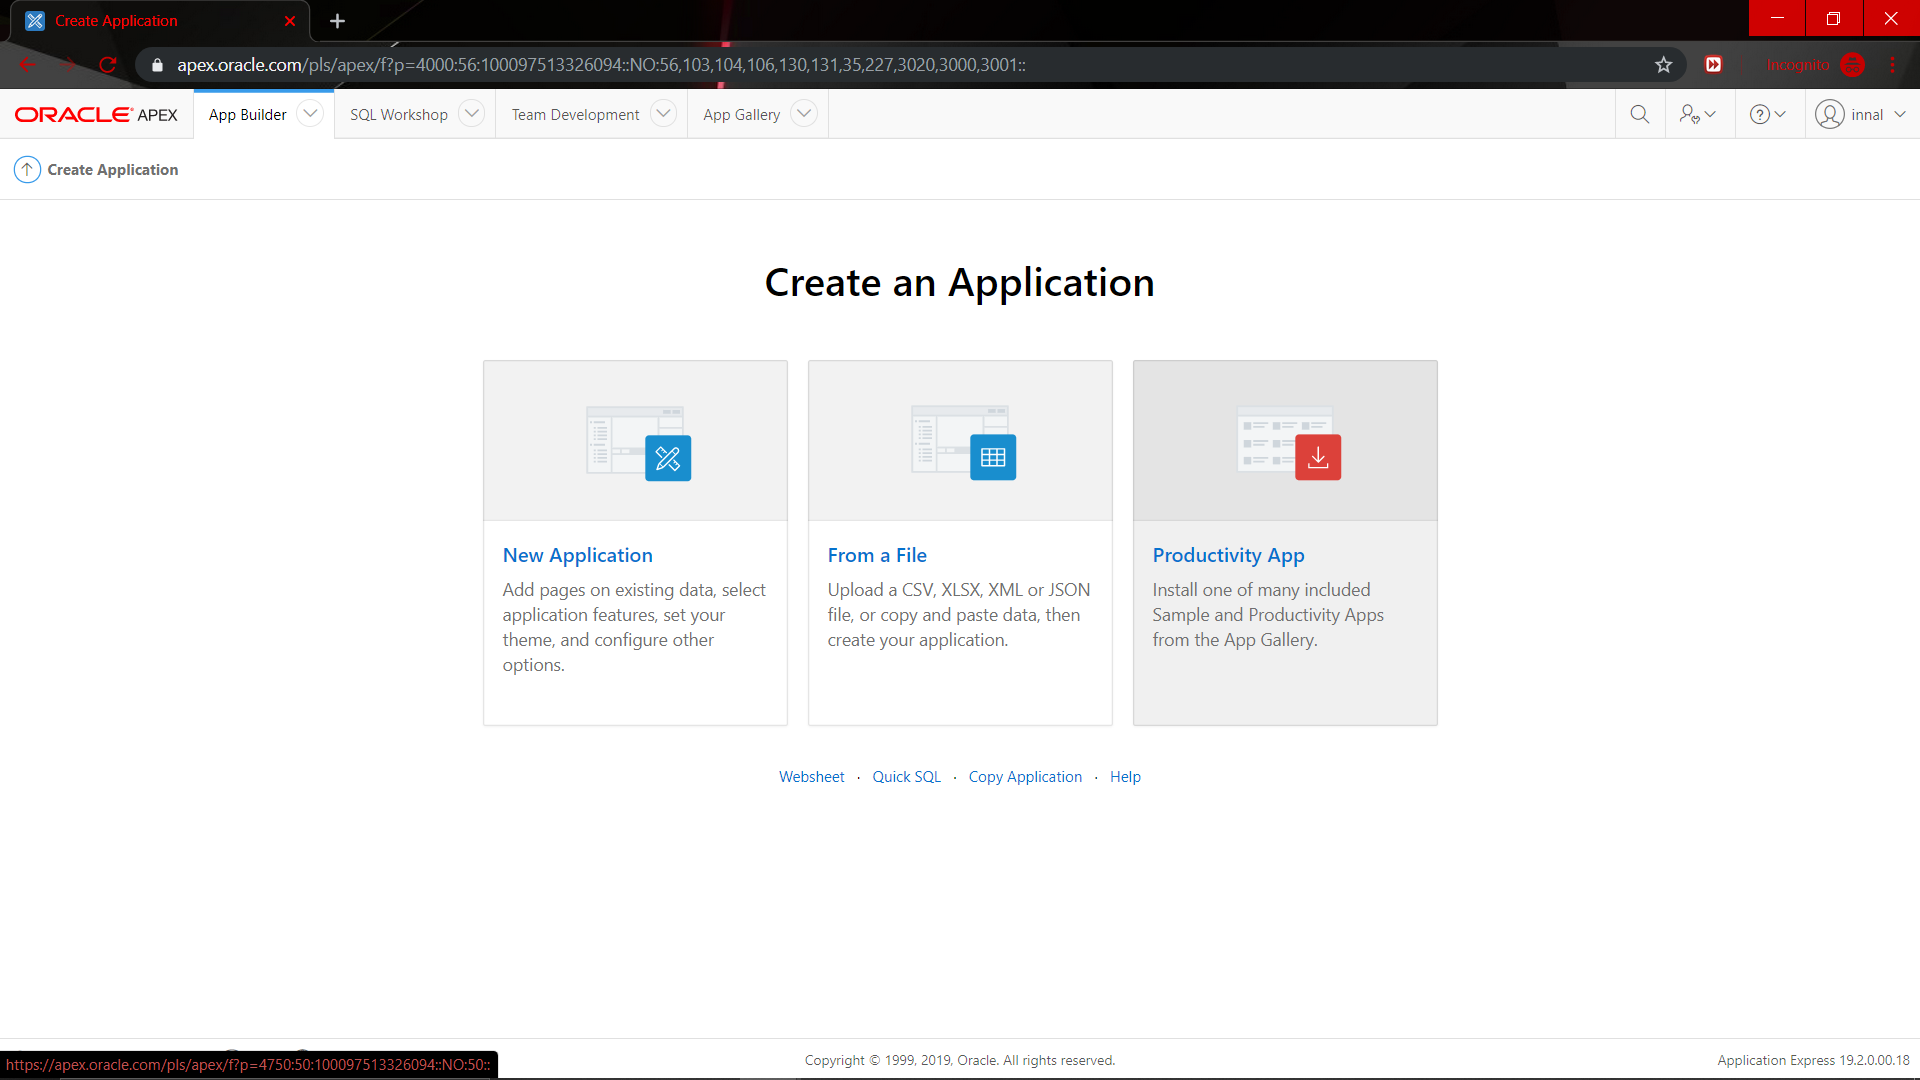
\includegraphics[scale=0.2]{Apex/64.png}
    \end{center}
    
     \item Lalu isikan namanya dan klik add page dan pilih yang interaktif report 
	\begin{center}
    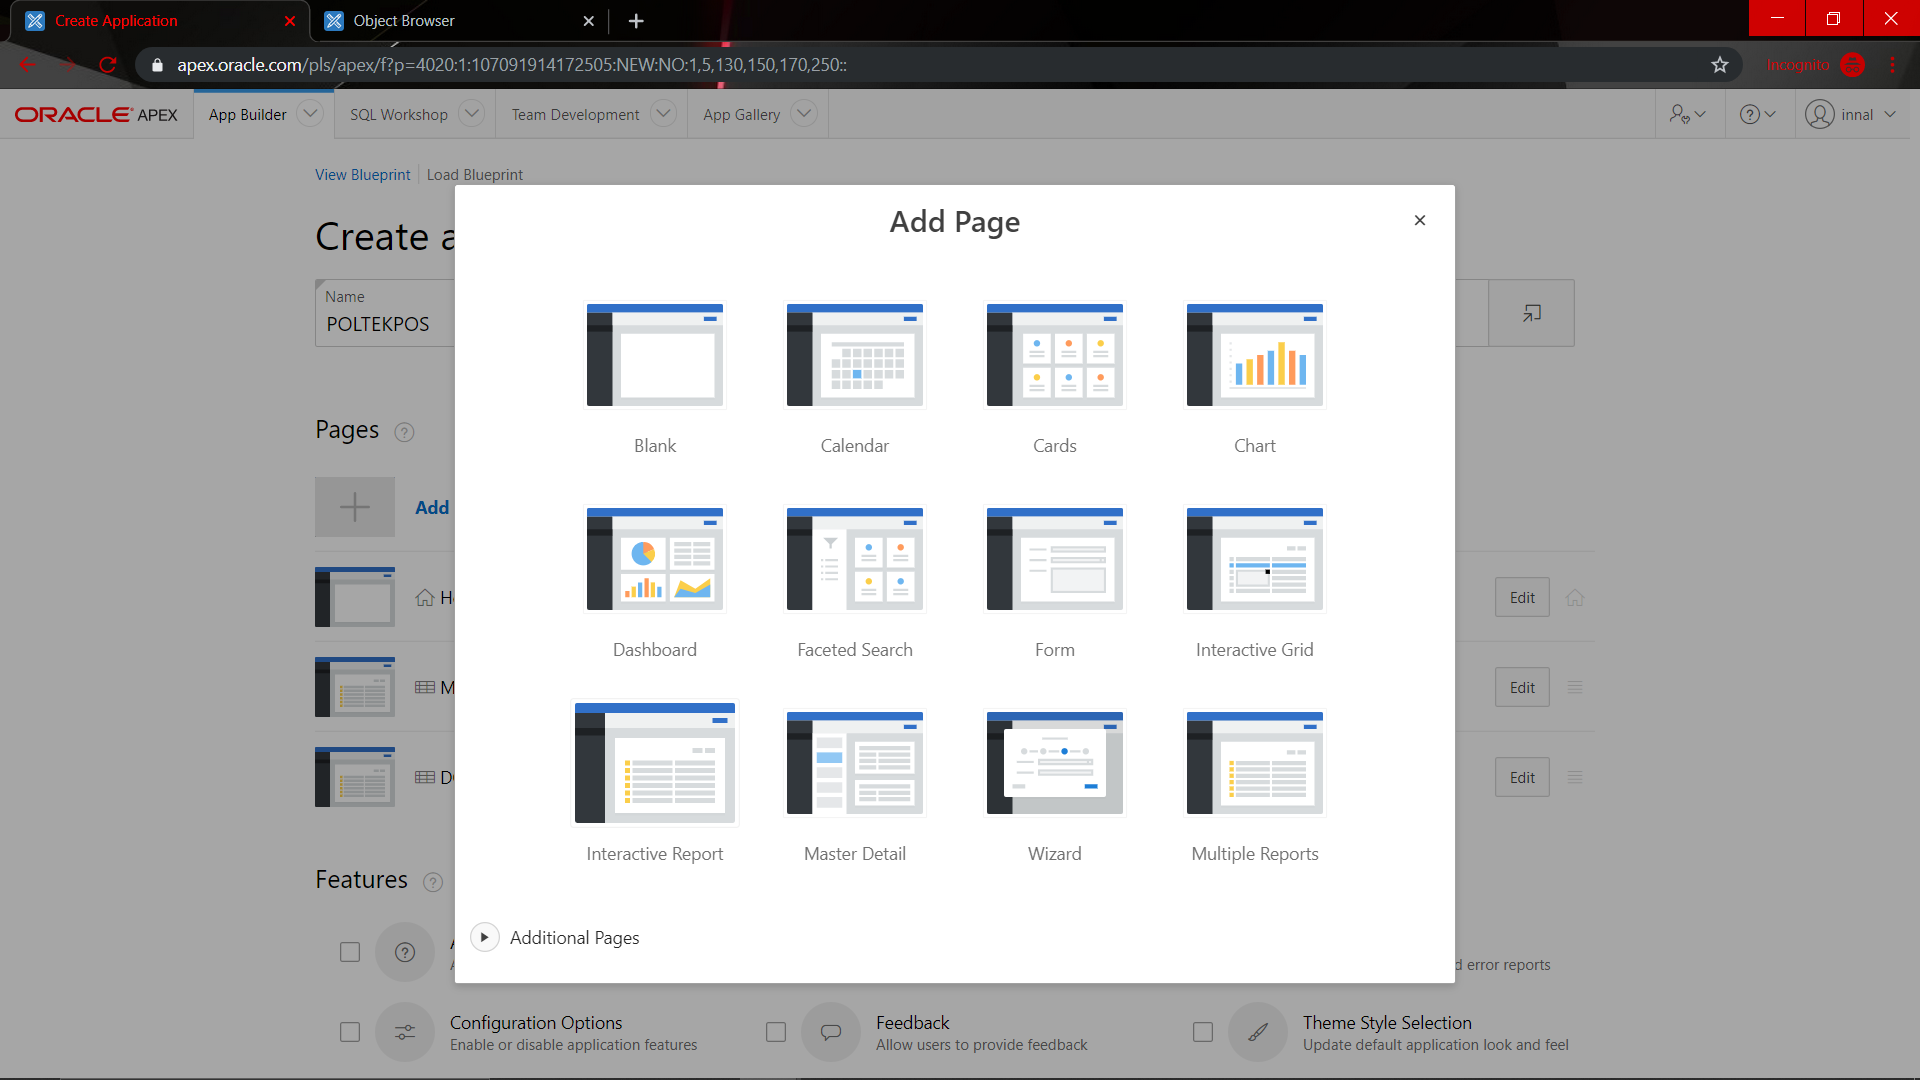
\includegraphics[scale=0.2]{Apex/65.png}
    \end{center}
    
     \item Kemudian isikan page name dan pilih tabel yang akan digunakan dengan cara tabel tabel or view pada bagian sebelah kanan kemudian klik add page. Ulangilah seperti langkah tersebut dengan memasukkan tabel mahasiswa, dosen jadwal, dan nilai
	\begin{center}
    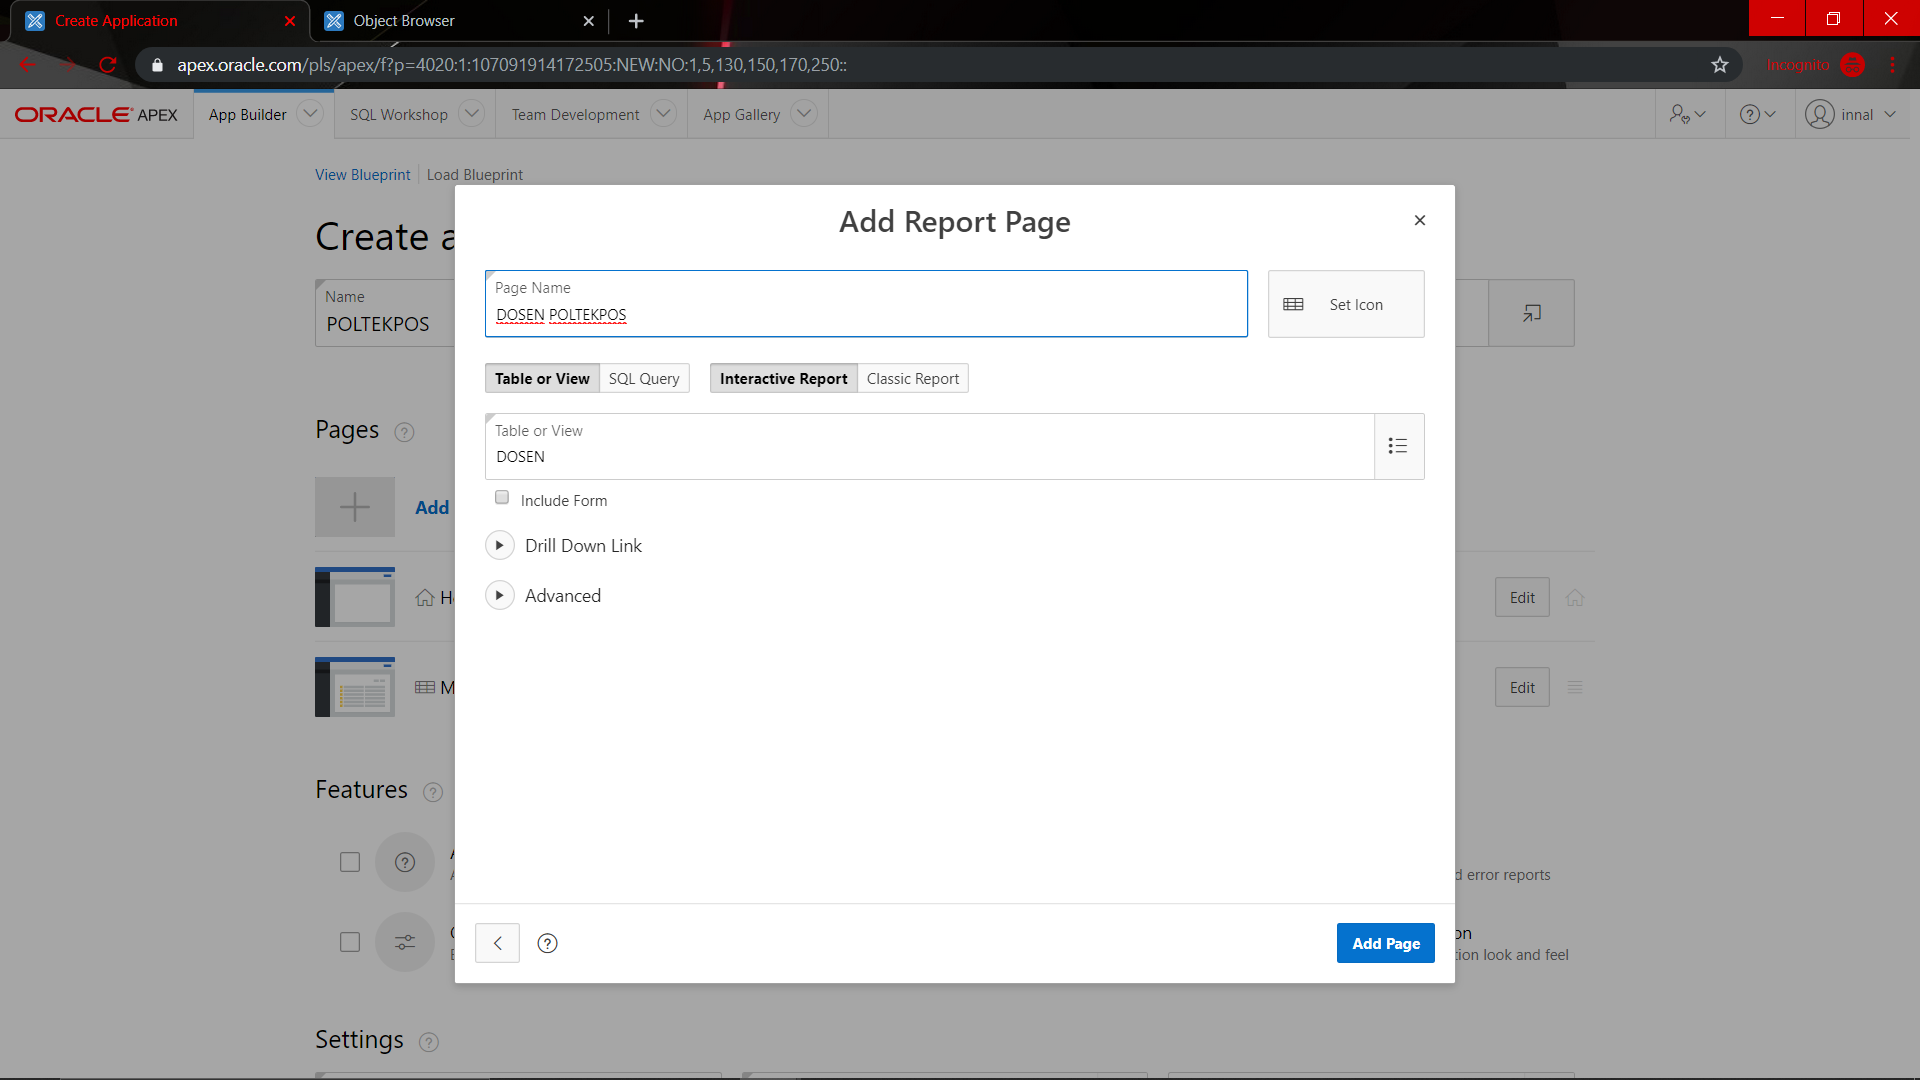
\includegraphics[scale=0.2]{Apex/66.png}
    \end{center}
    
     \item Kemudian pilih add page lagi,isikan page name "JADWAL lalu klik SQL query dan ketiklah pada SQL query seperti dibawah ini. kemudian klik add page
	\begin{center}
    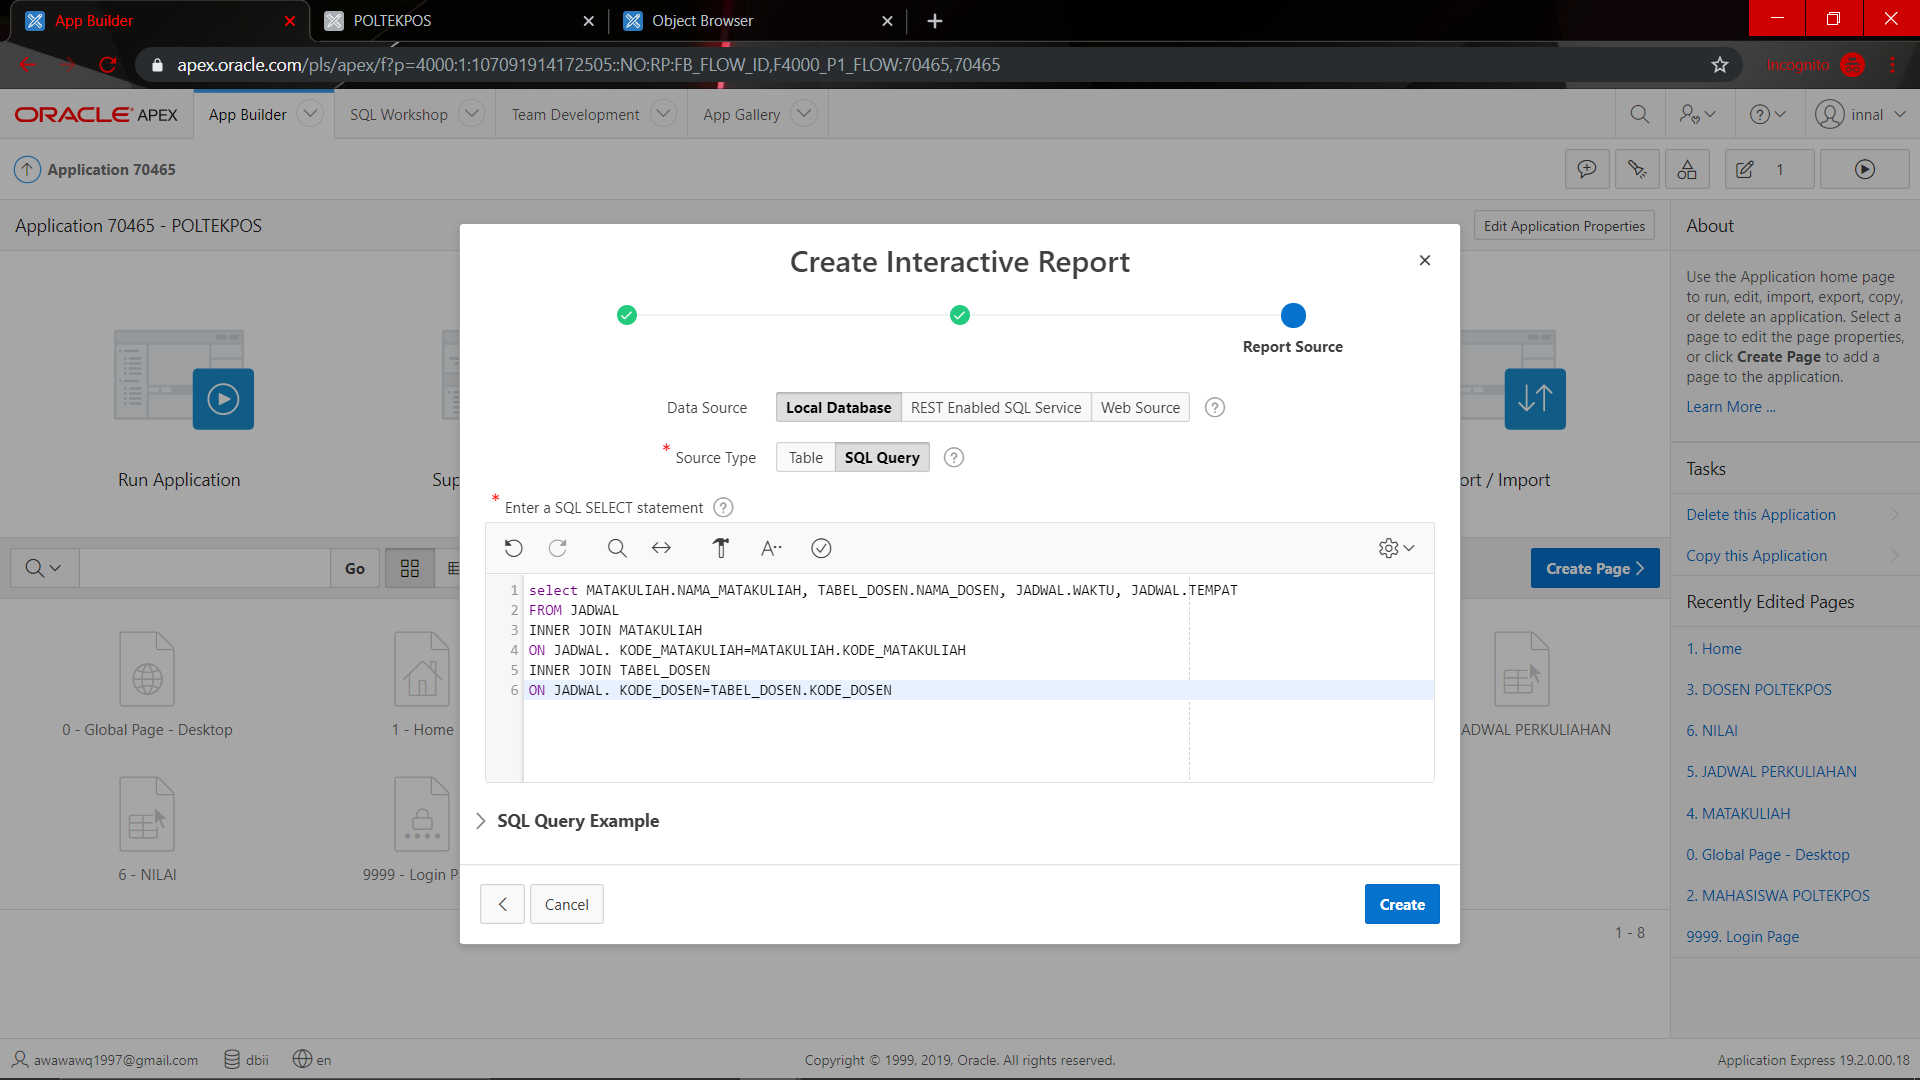
\includegraphics[scale=0.2]{Apex/69.png}
    \end{center}
    
     \item Kemudian create application seperti gambar dibawah ini
	\begin{center}
    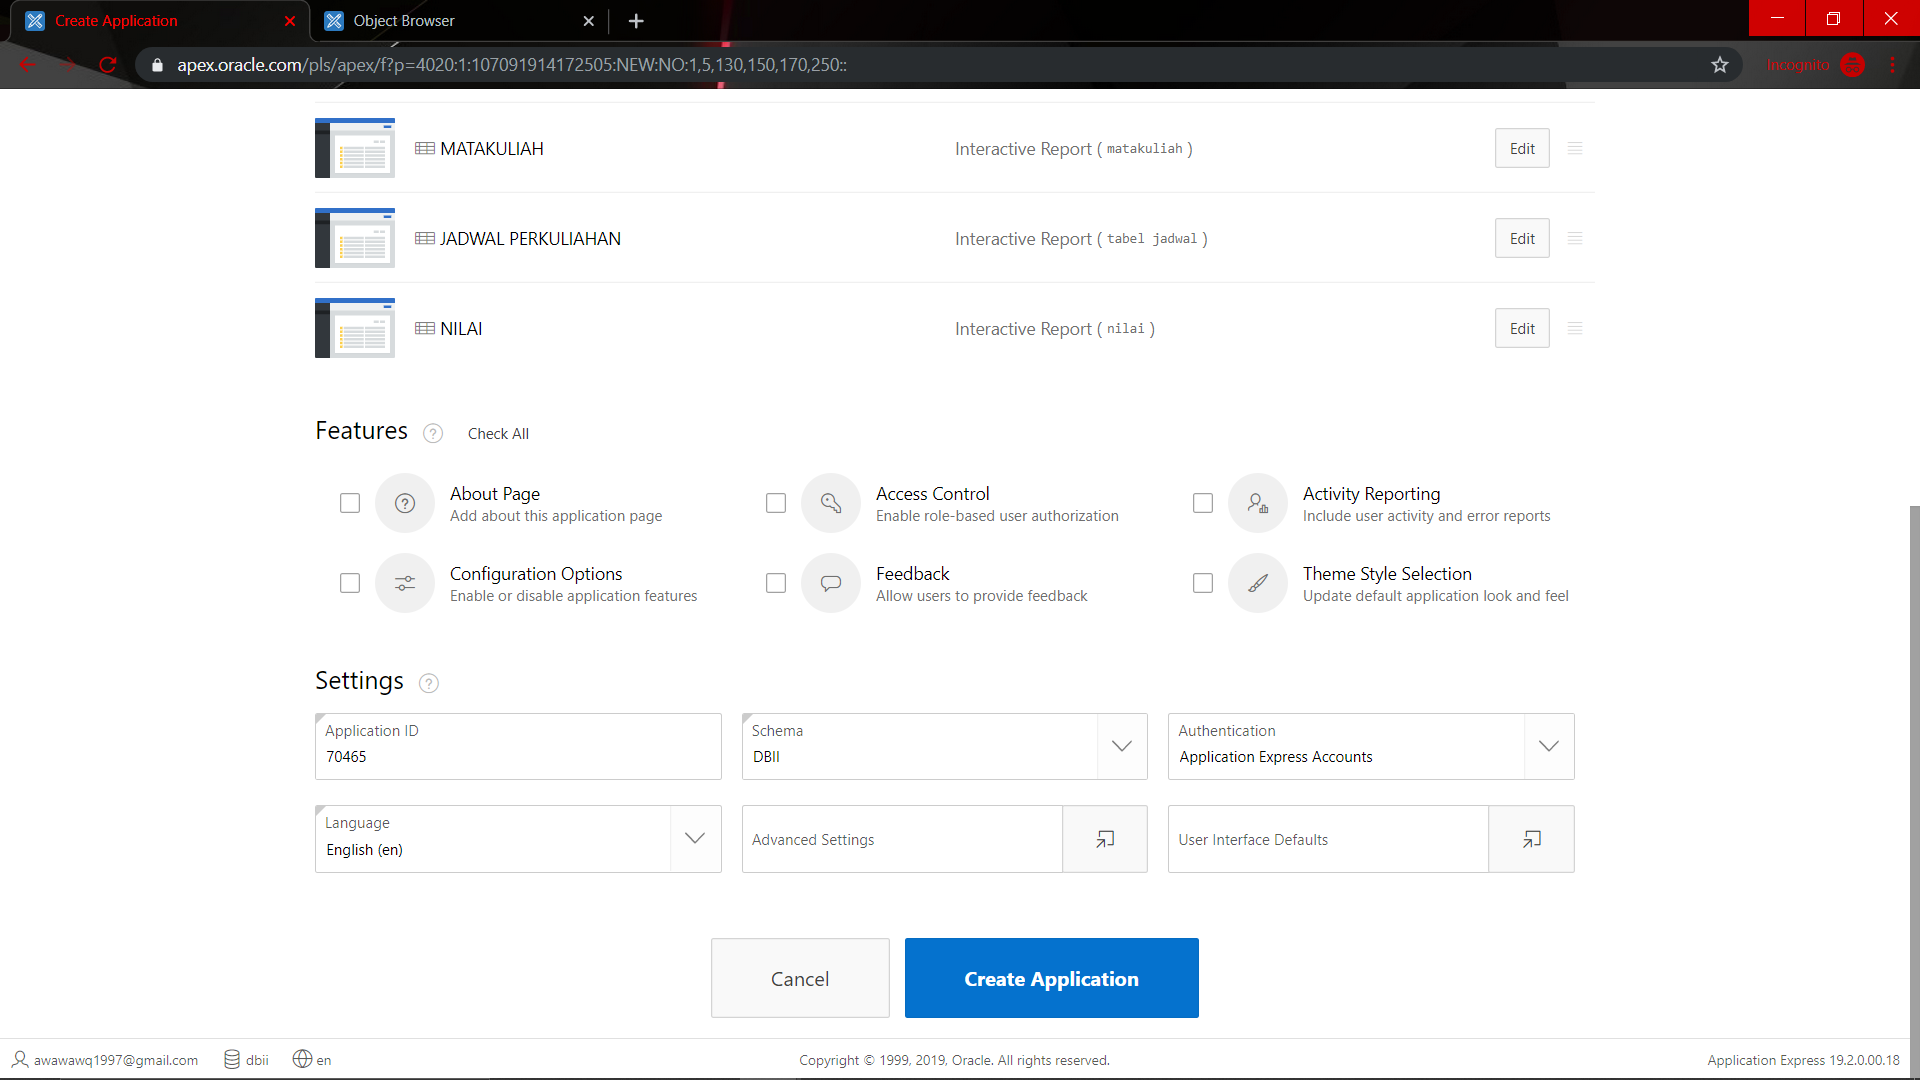
\includegraphics[scale=0.2]{Apex/73.png}
    \end{center}
    
     \item Setelah itu Run Application seperti gambar dibawah ini
	\begin{center}
    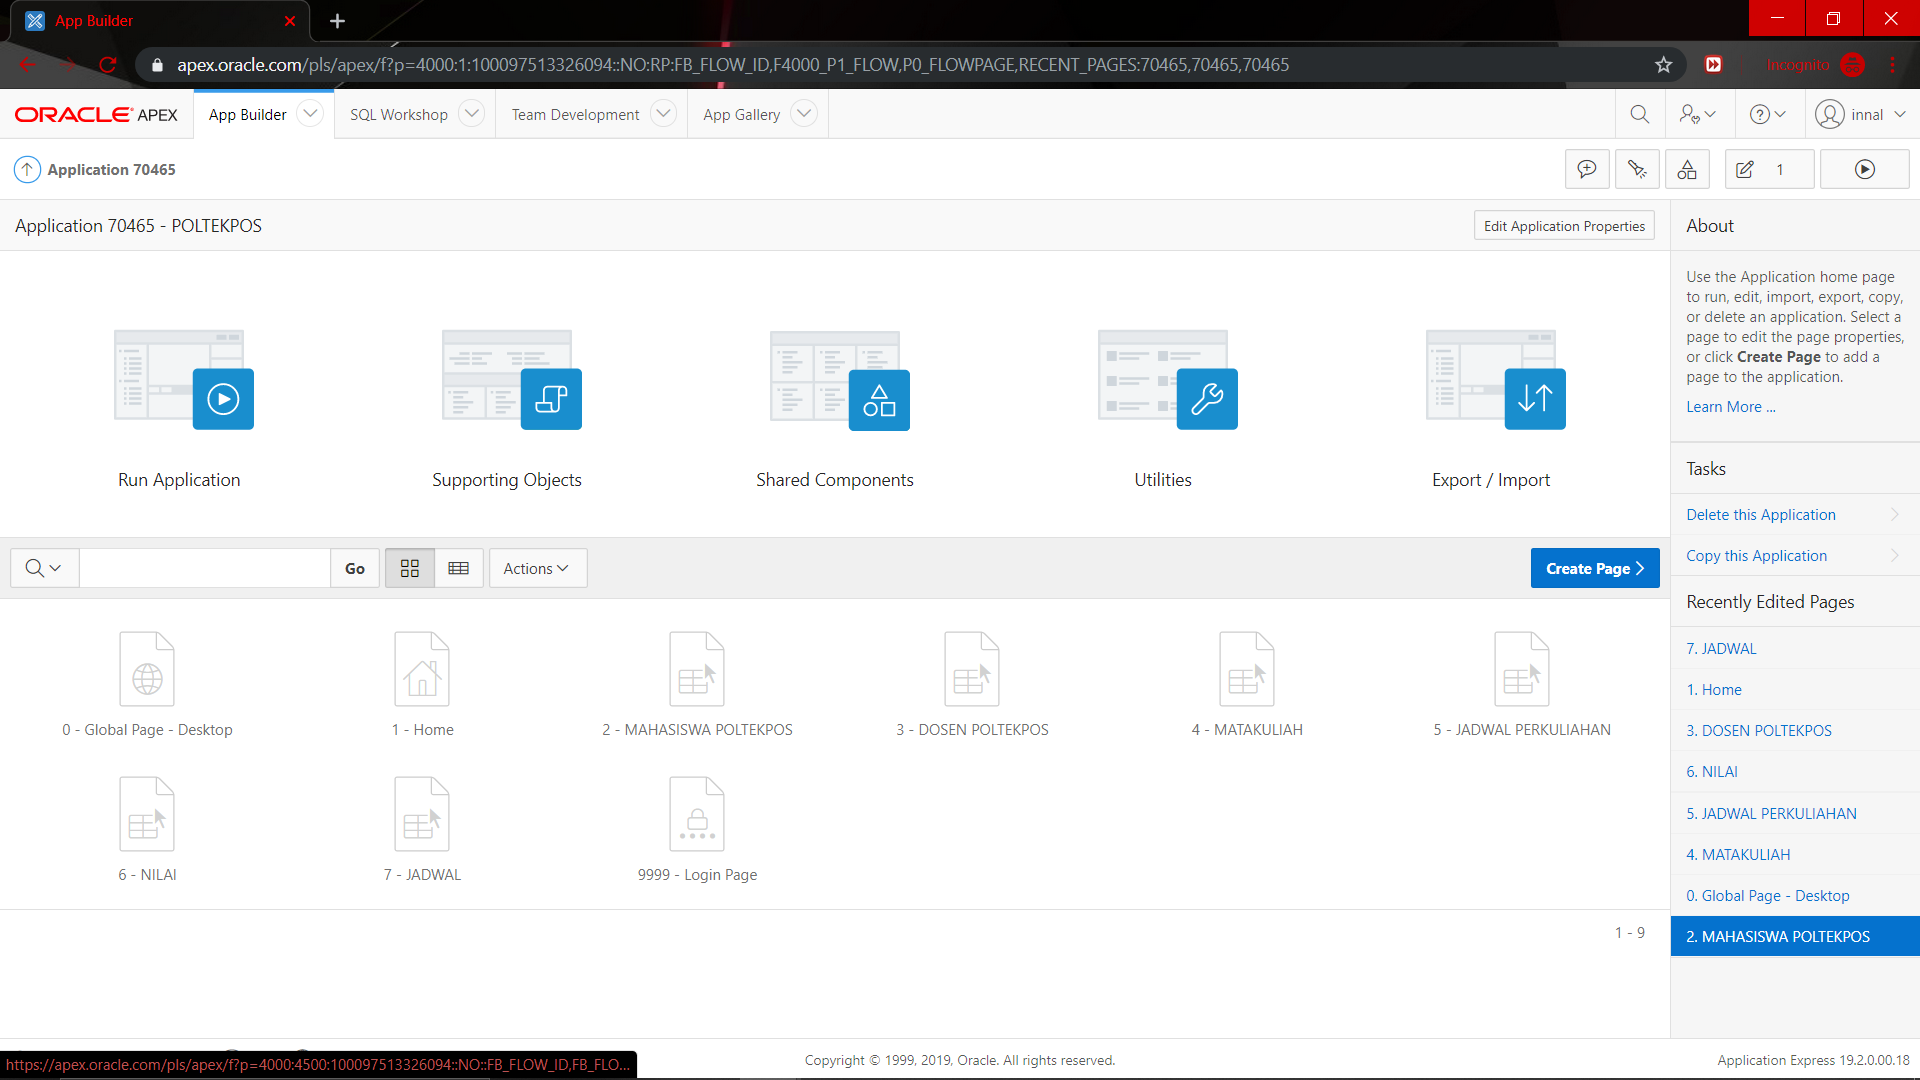
\includegraphics[scale=0.2]{Apex/74.png}
    \end{center}
    
     \item Kemudian akan muncul seperti gambar dibawah ini kalau sudah selesai semuanya
	\begin{center}
    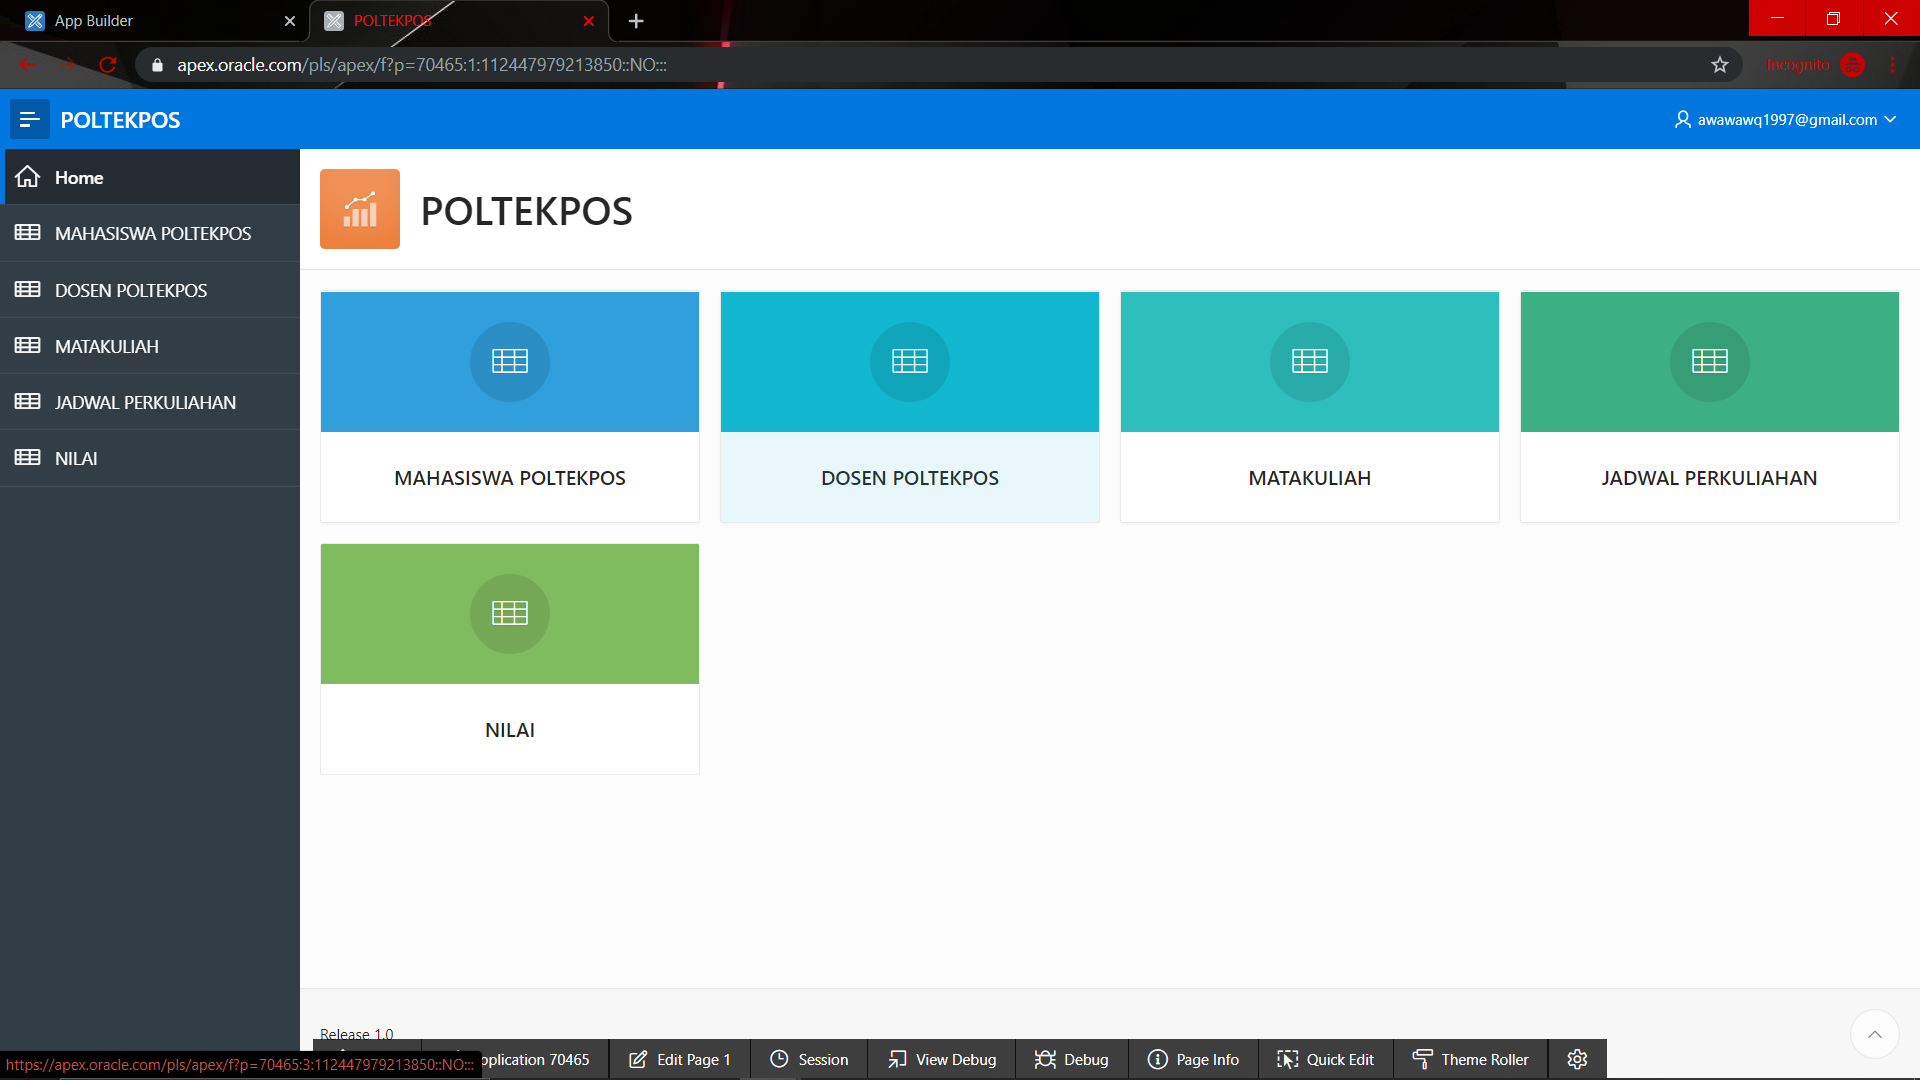
\includegraphics[scale=0.2]{Apex/76.png}
    \end{center}
    
    \item Workspace: DBII
    \item USERNAME : awawawq1997@gmail.com
    \item Password : kinoyku123
    
     
     

\end{enumerate}
